\documentclass[12pt,MSc,wordcount,twoside]{muthesis}
% The regulations say that 12pt should be used
% Change the MSc option to MPhil, MRes or PhD if appropriate

\usepackage{verbatim}
\usepackage{graphicx}
\usepackage{url} % typeset URL's reasonably
\usepackage{listings}
\usepackage{amsmath}
\usepackage{pslatex} % Use Postscript fonts
%\usepackage{subcaption}
\usepackage{subfig}
\usepackage{lipsum}
\usepackage{algorithm}
\usepackage[noend]{algpseudocode}

\makeatletter
\def\BState{\State\hskip-\ALG@thistlm}
\makeatother
\algnewcommand\algorithmicforeach{\textbf{for each}}
\algdef{S}[FOR]{ForEach}[1]{\algorithmicforeach\ #1\ \algorithmicdo}
\DeclareMathOperator{\sign}{sign}

\newenvironment{breakablealgorithm}
{% \begin{breakablealgorithm}
	\begin{center}
		\refstepcounter{algorithm}% New algorithm
		\hrule height.8pt depth0pt \kern2pt% \@fs@pre for \@fs@ruled
		\renewcommand{\caption}[2][\relax]{% Make a new \caption
			{\raggedright\textbf{\ALG@name~\thealgorithm} ##2\par}%
			\ifx\relax##1\relax % #1 is \relax
			\addcontentsline{loa}{algorithm}{\protect\numberline{\thealgorithm}##2}%
			\else % #1 is not \relax
			\addcontentsline{loa}{algorithm}{\protect\numberline{\thealgorithm}##1}%
			\fi
			\kern2pt\hrule\kern2pt
		}
	}{% \end{breakablealgorithm}
		\kern2pt\hrule\relax% \@fs@post for \@fs@ruled
	\end{center}
}

% Uncomment the next line if you want subsubsections to be numbered
%\setcounter{secnumdepth}{3}
% Uncomment the next line if you want subsubsections to be appear in
% the table of contents
%\setcounter{tocdepth}{3}

% Uncomment the following lines if you want to include the date as a
% header in draft versions
%\usepackage{fancyhdr}
%\pagestyle{fancy}
%\lhead{}  % left head
%\chead{Draft: \today} % centre head
%\lfoot{}
%\cfoot{\thepage}
%\rfoot{}

\begin{document}
% Uncomment the following lines to leave out list of figures, tables
% and copyright until final printing
%\figurespagefalse
%\tablespagefalse
%\copyrightfalse

\title{Analysis of Stock Market\\
  Using Complex Networks\\
  and Machine Learning}
\author{Lingjie Zhang}
\principaladviser{Eva Navarro-López}

\beforeabstract

\prefacesection{Abstract}
\abstracttitle
% Single spacing can be turned on for the abstract
%
{\singlespacing
	% EIO pathway -- machine learning pathway
Due to the complexity of financial market and the interconnectedness and interdependencies of industry sectors in the economy, the price returns of each coupling stocks might have certain underlying economic link. Such behaviours can hardly be explained by traditional financial models and theories. This thesis study on the construction and topological properties of US study stock market with complex networks theory. In order to determine the directions of edges in the stock network, we first used the machine learning technique to predict the Granger causalities of the price return series between all stock pairs while concluded with unsuccessful results. In addition, another method of using economical transactions of Economic Input-Output (EIO) from Bureau of Economic Analysis (BEA) is proposed. The constructed directed-unweighted stock network is partitioned in communities and compared with Erdős–Rényi (ER) random network and Watts-Strogatz (WS) small-world network with the same number of nodes and edges and the constructed directed-weighted stock network is compared with undirected-weighted stock network which is constructed by the method of correlation coefficient of stock price return series as previous researches conducted. Further, through analysing the topological properties including out-degree and out-strength distribution, efficiencies, betweenness centrality and clustering coefficient of both of the directed stock networks, we find that the main topological properties such as small-world feature and power-law distribution of degrees are still exist as the conventional undirected stock networks follow. Suggestions towards financial market investment are provided based on the results of the study.
}



\afterabstract

\prefacesection{Acknowledgements}
I would like to thank...
\afterpreface

\tableofcontents

% These include the actual text
\chapter{Introduction}
\section{Motivation}
Financial markets are complex systems, the interconnectedness and interdependencies of industry sectors in the economy are highly inter-coupled with strong correlations with stock price fluctuations, i.e., the price returns of each coupling stocks underlying certain economic link, e.g. two companies that manufacture similar products, or both in one supply chain. Such behaviours can hardly be explained by traditional financial models and theories.

During recent times, weighted but undirected complex network models have been applied to study the correlations of stock prices. Prevailing approach is using companies as nodes, and correlations between each pair of stock price series, return series, or fluctuation patterns as links, e.g., much of the previous researches have proved the represented complex networks of worldwide stock markets are scale-free and small-world~\cite{cnsm, perspective}.

Theoretically, directed complex network for stock market can be achieved therefore more potential information can be produced which is helpful for investment decision and financial market supervision. Conducting Granger causality test between stock pairs is straightforward but not feasible due to the heavy- precondition and time-complexity in programme. Compared to the large order of magnitude of total stock pairs, manually calculated Granger causalities are too less to be used as training samples. Enlightened by the recent work by Jean et al. [3] which uses transfer learning and noisy proxy information performed very well at predicting poverties, demonstrating that machine learning techniques is powerful to be applied in a setting with limited training data, so an exploration towards the directed network of stock market is motivated in this project, combines machine learning techniques, transfer learning, individual stock features, and empirical data of Industry Economic Accounts (IEAs) from Bureau of Economic Analysis (BEA) in the US to predict Granger causality of coupling US stocks. Therefore, a directed weighted complex network (DWCN) is constructed by considering companies as nodes, correlations of abnormal stock returns (alpha) as weights of links, and predicted Granger causalities as the indications of directions of links.

% hence a new perspective is needed

The goal of this project is to reveal the Granger causality of price return series and utilise them into the topological analysis and visualisation of DWCN as so far no previous work has attempted to construct a directed network about stock price. In addition, suggestions for stock market are provided according to the results and findings.

The outline of this document is as follows. In Section 2, specific objectives and deliverables are listed. In Section 3, relevant previous researches on financial market, complex networks, and machine learning are reviewed. Section 4 describes the analytical methods. Ethics and professional considerations and risk considerations are respectively discussed in Section 5 and 6. Section 7 describes project evaluation approaches and finally, planning Gantt chart is presented in Section 8.

% In the viewpoint of directed networks, the analysis of stock complex network can provide new 

\section{Objectives and deliverables}
% in list
% To - ...

The goal of this project is to construct a directed complex network using economical industrial transaction data and stock price data to depict the US stock market by means of topological properties analysis, community detection and visualisation. Same-sized directed Watt-Strogats small-world network and random networks are generated for the purpose of comparison. This paper will explore whether the conclusions are consistent with the undirected complex network researches.

\vline

Objectives produced:

\begin{itemize}
	\item The individual entries are indicated with a black dot, a so-called bullet.
\end{itemize}

\vline

Deliverables produced:

\begin{itemize}
	\item Stock counts by industries.
	\item Matrix of EIO transaction flows.
	\item Heatmap of combinations of thresholds of directed demands and directed requirements flows and correlation coefficients.
	\item Two benchmarking networks: directed Watts-Strogatz small-world network and directed Erdős–Rényi random network.
	\item Directed-unweighted and directed-weighted stock network.
	\item Topological properties of studied networks.
	\item Community partition of directed-unweighted stock network.
	\item We plan to produce a research paper to submit to a journal. We are thinking of journals like:  \textit{Physica A, Journal of Mathematical Finance, Journal of Applied Mathematical Finance, Applied Network Science}.
\end{itemize}

\section{Proposed methodology}
% summary and put a diagram of the part of my thesis



\section{Summary of results}
% list
This paper finds the directed-weighted stock network is consistent with the undirected-weighted networks about some important topological properties in previous studies, i.e, they are both small-world and scale-free. The study on community detection suggests "livelihood" and "production" are the dominant and influential sectors in the stock market and the "finance" sector has extremely strong internal connections. This paper also finds there is significant negative relationship between standard deviation of stock price return and its corresponding betweenness centrality. The theoretical and practical contributions of aforementioned findings are discussed.

\section{Outline of the thesis}
The rest of this thesis is organised as follows. Chapter~\ref{cpt:back} discusses the development of quantified financial analysis for stock markets and the application of complex theories of complex networks towards stock markets. The subsequent chapters of methodologies introduce the critical analytical methods implemented in the research by this paper. Detailed outcomes are then illustrated in Chapter~\ref{cpt:result}. Finally, the findings and conclusions are discussed in Chapter~\ref{cpt:conclude}.

% 建立投资组合,不仅需要时间序列上的不相关性,也需要经济上潜在的不相关性。edge的weight代表价格时间序列上的不相关性,而方向代表经济上的。从而对建立有效的投资组合提供建议。
\chapter[Short Chap title]{Background}
The revolutionary who pioneered the theory of portfolio, Markowitz \cite{portfolio} proposed the mean-variance model and established a clear mathematical definition of the two vague concepts of risk and return. Sharp \cite{equilibrium} and Linter \cite{diversification} added two key assumptions based on the mean-variance model to enable the portfolio mean-variance valid, forming a capital asset pricing model (CAPM) with the support of economic theories. The CAPM believes that only non-dispersible systemic risks can be compensated off, while non-systematic risks can be eliminated by effectively decentralised investments. Investors could only assume systemic risks through decentralised investment. The systematic risk of a single security or portfolio can be characterised by beta, which represents the extent to which a single security or portfolio is affected by the overall market volatility.\\[2mm]
Worldwide scholars had been actively conducting empirical tests towards the practicality of the CAPM then, while early results show that beta is able to explain return movements of stocks. However, in the late 1970s, some empirical studies upon the CAPM began to show that a large part of the changes in the stock returns cannot be explained by beta, with increasingly market return anomalies were found.\\[2mm]
Researchers had proposed models and theories considering the individual stock features to explain. For instance, Fama and French \cite{riskfactors, anomalies} proposed a three-factor model based on the inter-temporal capital asset model (ICAPM) \cite{intertemporal} and the arbitrage pricing theory (APT) \cite{options}, which reveals a large part of the cross-section of the stocks’ average return that cannot be explained by CAPM, can be explained using firm size, book-to-market equity ratio, and overall market return.\\[2mm]
While traditional stock pricing models still capture limited forms of financial behaviour, the premises of standard financial theory contradict the modern notion of financial markets are complex systems \cite{financialcomplex}, by which many statistical niceties such as stationarity no longer can be taken for granted. Recent researches have implemented the network theory to reveal the underlying factors of price movements. Huang et al. \cite{chinesenetwork} implemented the threshold method to build ’s correlation network in China's A-Share stock market and studied the networks topological properties and topological stability. Namaki et al. \cite{genuine} utilised Random Matrix Theory (RMT) to specify the biggest eigenvector in the complex network of price correlations. Yu \cite{visibility} studied the evolution of gold price from a network perspective using the visibility network approach. Chopra and Khanna \cite{intercd} developed a framework which associates the economic input–output (EIO) model with techniques for understanding interdependencies and interconnectedness in the economy of US, based on complex networks theory. Boginski et al. \cite{statisticalanalysis} identified cliques and independent groups among stock networks. Chen et al. \cite{profitable} studied the inter-stock and inter-industry effects towards stock returns based on the topological properties of a complex network of correlations.\\[2mm]
In a nutshell, prevailing complex network approaches to analyse stock markets are almost all about investigating weighted or unweight but undirected networks. To the best knowledge of mine, no previous work has attempted to construct a directed network so far.

% Local Variables: 
% mode: latex
% TeX-master: "report"
% End: 

\chapter[Short Chap title]{Benchmarking networks}
Specify the number of nodes $N$, the mean degree $K$ (assumed to be an even integer), and a special parameter $\beta$, satisfying $0\leq \beta \leq 1$ and $ N\gg K\gg \ln N\gg 1$ $N\gg K\gg \ln N\gg 1$, the model constructs an undirected graph with $N$ nodes and $\frac{NK}{2} \frac {NK}{2}$ edges in the following way.

\begin{algorithm}[H]
	\caption{WattsStrogatzSmallWroldNetwork}\label{alg:smallworld}
	\begin{algorithmic}[1]
		\Procedure{GenerateSmallWorldNetwork}{\textit{nNodes, p0, beta}}
		\State $\textit{Dmax} \gets \textit{nNodes \% 2}$ 
		     circulant(D)/Dmax
		
		\State \textbf{return} \textit={A}
		\EndProcedure
	\end{algorithmic}
\end{algorithm}

\chapter{Community detection}
\section{Introduction}
This paper considers a theoretic concept of modularity-based community detection method for directed graphs to recognise natural faults occur in the stock network along which it partitions. Community detection is applied for further understanding to the overall pattern of economical and stock price relations of listed companies.

While there are many methods to identify communities in undirected graphs, the community detection method used in this paper is for the directed graphs proposed by Leicht and Newman~\cite{PhysRevLett.100.118703}, which based on modularity optimisation method. Modularity optimisation method identifies communities by maximizing the modularity $Q$, which is defined as:
\begin{eqnarray}
Q=(\textit{fraction of intra-community edges}) - (\textit{expected fraction of such edges})
\end{eqnarray}

It signifies that a community is figured when the number of edges inside the community is more than the expected number on the basis of chance. As a result, modularity-based community detection maximised intra-community density and minimised inter-community density. While the complexity of modularity optimisation is NP-complete problem, this paper uses the spectral optimisation methodology, which finds the best partition of the directed US stock network by the following expression of $Q$:
\begin{eqnarray}
Q=\frac{1}{m}\sum_{ij}{\left[A_{ij}-\frac{k_i^{\text{in}}k_j^{out}}{m}\right]}\delta_{c_i,c_j}
\end{eqnarray}

where $A_{ij}$ is defined to be $1$ if there is an edge from $j$ to $i$ and $0$ otherwise. $k_i$ is the in-degree for node $i$, $k_j$ is the out-degree for node $j$, $m$ is the total number of edges in the network. $\delta$ is the Kronecker delta symbol that is $1$ if nodes $i$ and $j$ are in the same community, i.e., $C_i=C_j$, and $0$ otherwise. Spectral optimisation technique for modularity maximisation assigns nodes to different communities based on the sign of the eigenvector, corresponding to the largest positive eigenvalue of the modularity matrix \textbf{B}, whose elements are:
\begin{eqnarray}
B_{ij}=A_{ij}-\frac{k_i^{in}k_j^{out}}{m}
\end{eqnarray}

This paper applies the repeated bisection graph-partitioning algorithm in the cause of community detection according to Leicht and Newman~\cite{PhysRevLett.100.118703}. This approach begins with partition the network in two and then repeating it while optimising for the maximum modularity score of the communities. A preferred partition of a network results in a higher modularity score, therefore the modularity $Q$ is maximised over all possible partitions of the stock network to detect communities of listed companies.

The following algorithm describes the details about the partitioning process and maximising modularity score in community detection. The functions of calculating modularity and subdividing node group are called repeatedly over iterations until no further increment of the overall modularity score.

\begin{algorithm}[H]
	\caption{Community detection}\label{alg:communitydetection}
	\begin{algorithmic}[1]
		\Procedure{Community}{\textit{G, nNode, nEdge, EntireModMat, EntireNodeSpace}}
		\Procedure{CalDeltaQ}{\textbf{s}, \textbf{B}}
		\State \textbf{return} \emph{$\textit{Q} \gets \text{1 / (4 * \textit{nNode})} * \textbf{s}^T(\textbf{B}+\textbf{B}^T)\textbf{s}$}
		\EndProcedure
		\Procedure{UpdCommunityAssignment}{\textit{NodeSpace}, \textit{UpdAssign}}
		\State $\textit{Mark1, Mark2} \gets \max( \textit{Assignment})+1, \max( \textit{Assignment})+2$
		\ForEach {$\textit{node} \in \textit{NodeSpace}$}
		\If {$\textit{node} \in \textit{UpdAssign} > 0$} {$\text{node of } \textit{Assignment} \gets \emph{Mark1}$}
		\EndIf
		\If {$\textit{node} \in \textit{UpdAssign} < 0$} {$\text{node of } \textit{Assignment} \gets \emph{Mark2}$}
		\EndIf
		\EndFor
		\State \textbf{return} \emph{Assignment}
		\EndProcedure
		\Procedure{SubdivideCommunity}{\textbf{B}}
		\State $\textit{SymmetricMatrix} \gets  \textbf{B}+\textbf{B}^T$
		\State $\textit{eigv} \gets \text{eigenvector as }\max(eigenvalues) \text{ in } \textit{SymmetricMatrix}$
		\State \textbf{return} $\sign(\textit{eigv})$
		\EndProcedure
		\Procedure{CalModularity}{\textit{assignment}}
		%\State Initilize $Q \gets 0$
		\ForEach {$\textit{node1} \in \textit{Nodes of G}$}
		\ForEach {$\textit{node2} \in \textit{Nodes of G}$}
		\If {$\textit{assignment} \text{ of }  \textit{node1} \gets \textit{assignment} \text{ of } \textit{node2}$}
		\State $Q \gets Q + HasEdge - (\text{nIn}( \textit{node1}))*(\text{nOut}(\textit{node2}))/ (\text{nEdge})$
		\EndIf
		\EndFor
		\EndFor
		\State \textbf{return} \emph{$Q / (\text{nEdge})$}
		\EndProcedure
		\Procedure{GenModularityMatrix}{\textit{NodeSpace}, \textit{ModMat}}
		%\State Initilize $ModMat \gets \text{2-D matrix of } \textit{NodeSpace}$
		\ForEach {$\textit{node1} \in \textit{NodeSpace}$}
		\ForEach {$\textit{node2} \in \textit{NodeSpace}$}
		\State $\textit{B} \gets \textit{HasEdge} - (\text{nIn}( \textit{node1}))*(\text{nOut}( \textit{node2})/\text{nEdge})$
		\If {\text{Assignment of } \textit{node1} = \text{Assignment of } \textit{node2}}
		%\State Initilize $C \gets 0$
		\ForEach {$\textit{node} \in \textit{NodeSpace}$} {$C \gets C+\textit{HasEdge1}+\textit{HasEdge2}-(\text{nIn} (\textit{node1})*\text{nOut}(\textit{node})+\text{nIn}( \textit{node})*\text{nOut}(\textit{node1}))/\text{nEdge}$}
		\EndFor
		\EndIf
		\EndFor
		\EndFor
		\EndProcedure
		\Procedure{InterateBisection}{\textit{ModMat, NodeSpace}}
		\State $\textit{UpdAssign} \gets \text{SubdivideCommunity}(ModMat)$
		\State $\textit{DeltaQ} \gets \text{CalDeltaQ}(\textit{UpdAssign}, \textit{ModMat})$
		\If {$DeltaQ > 0$}
		\State $\textit{Assignment} \gets \text{UpdCommunityAssignment}(\textit{NodeSpace}, \textit{UpdAssign})$
		\ForEach {$\textit{side} \in \textit{UpdCommunityAssignment}$}
		\State $\textit{ModMat} \gets \text{GenModularityMatrix}(\textit{NodeSpace})$
		\State $\text{InterateBisection}(ModMat, NodeSpace)$
		\EndFor
		\EndIf 
		\EndProcedure
		\State $\text{InterateBisection}(EntireModMat, EntireNodeSpace)$
		\State \textbf{return} \emph{Assignment}
		\EndProcedure
	\end{algorithmic}
\end{algorithm}
\section{Summary}

\chapter[Short Chap title]{Empirical study and results}
\section{Data}
This paper considers 1,418 stocks of listing US companies that traded consecutively in the NYSE and NASDAQ stock market of US from January 4, 2016 to December 30, 2016 and uses daily closing price during this period.
% 写一下EIO数据的来源和时间

\section{Network construction}
This paper first calculated normalised direct requirement and normalised direct demand values for every sectors using formula~\ref{equ:eio_i} and formula~\ref{equ:eio_o} and cross-correlation coefficients between every stock pairs using formula~\ref{equ:corr}.

According to the figure~\ref{fig:eio_transaction_density}, the transaction densities decrease as threshold of normalised direct requirement and normalised direct demand increase, and their patterns are exactly similar with the same inflection point at around $threshold=0.136$ where the densities begin to decline. Therefore, the values of thresholds for normalised direct requirement and normalised direct demand are set to be same, i.e., $\theta_{DD}=\theta_{DR}=\theta_{EIO}$,  to filter the directed edges among the stock network.

\begin{figure}
	\begin{center}
		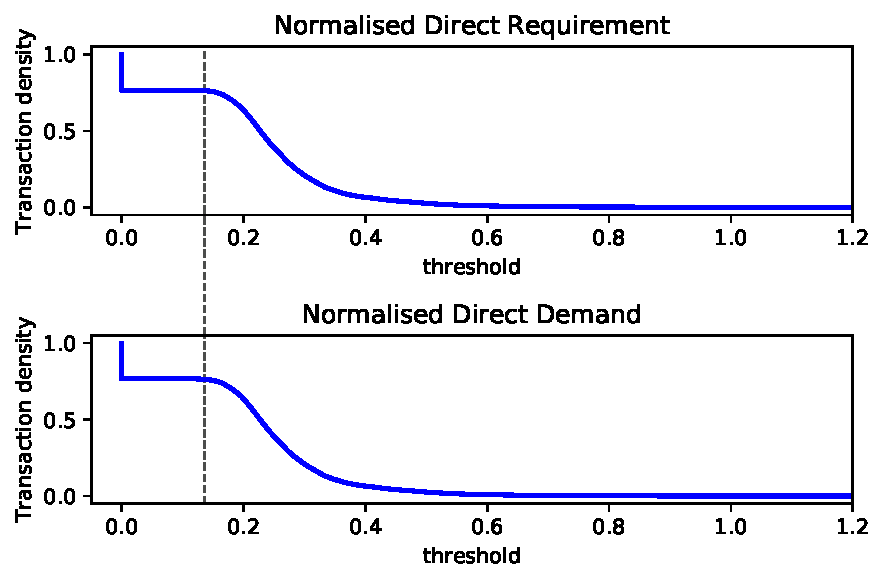
\includegraphics[width=14cm]{eio_transaction_density}
	\end{center}
	\caption{Transaction densities}
	\label{fig:eio_transaction_density}
\end{figure}

\begin{figure}
	\begin{center}
		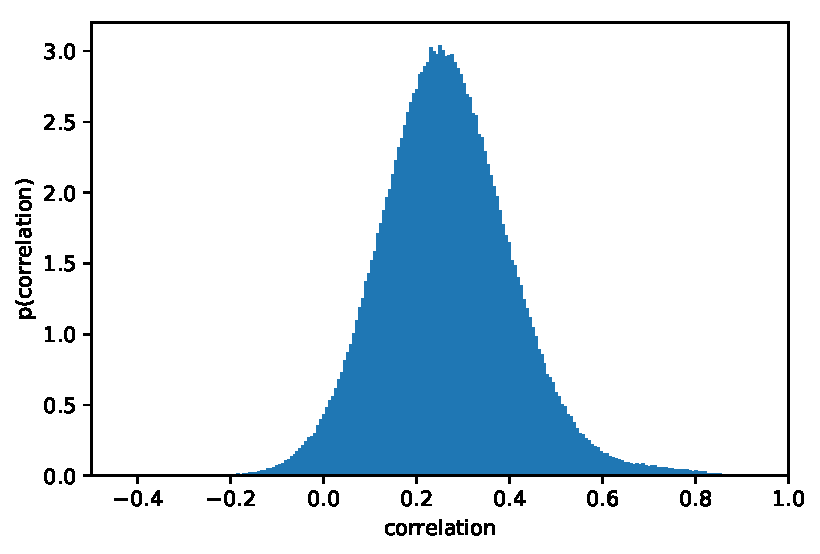
\includegraphics[width=14cm]{correlation_distribution}
	\end{center}
	\caption{Stock price return correlation coefficient distribution}
	\label{fig:correlation_distribution}  
\end{figure}

\begin{figure}
	\begin{center}
		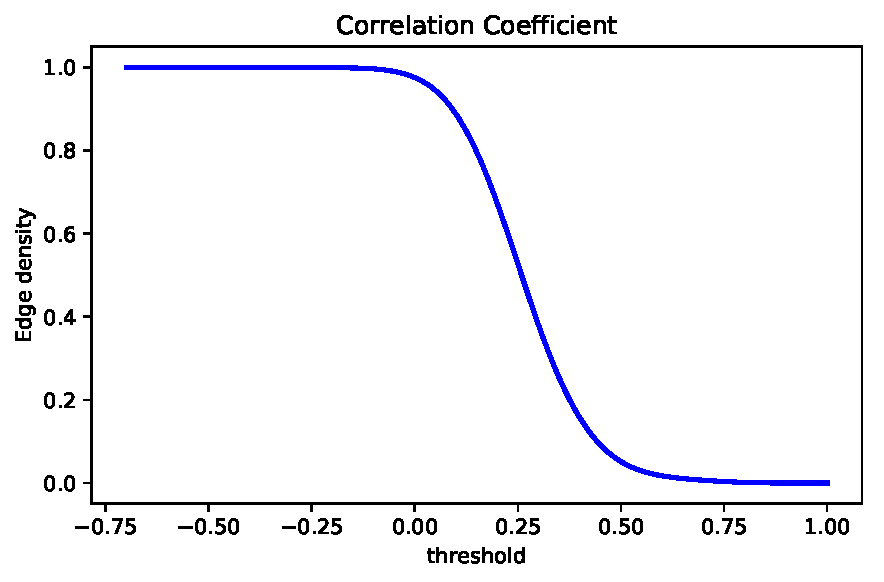
\includegraphics[width=14cm]{correlation_edge_density}
	\end{center}
	\caption{}
	\label{fig:correlation_edge_density}  
\end{figure}

Figure~\ref{fig:correlation_distribution} shows the distribution of stock price correlation coefficients has a shape complies to the normal distribution for the long tails. The correlation coefficients are vary from -0.687 to 0.977 with the mean of 0.265. It implies that the prices of most stocks traded in NYSE and NASDAQ usually fluctuate to the same direction.

% 拟合正态分布或t分布

\begin{figure}
	\begin{center}
		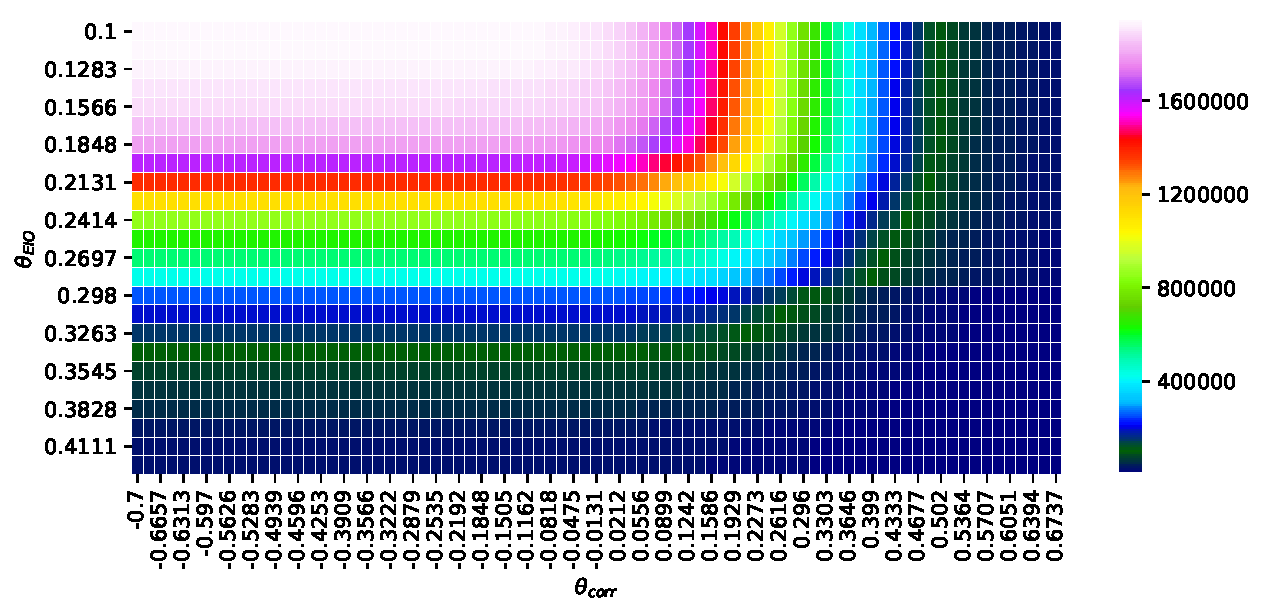
\includegraphics[width=15cm]{amounts_of_edges_threshold}
	\end{center}
	\caption{Numbers of directed edges per EIO-threshold and correlation-coefficient-threshold}
	\label{fig:amounts_of_edges_threshold}  
\end{figure}

Figure~\ref{fig:amounts_of_edges_threshold} shows the number of directed edges remain in the conditions of different value combinations of $\theta_{EIO}$ and $\theta_{corr}$. When both of the thresholds set to be minimal at their own value range, i.e., $\theta_{EIO}=0$ and $\theta_{corr}=-1$, the number of directed edges is $N\times(N-1)=2,009,306$, while $N$ indicates the total number of nodes. According to the figure~\ref{fig:amounts_of_edges_threshold}, the number of edges will be less than 100,000, in which case the network has a density of less than 5\%, if $\theta_{EIO}$ is larger than 0.3545 or $\theta_{corr}$ is larger than 0.5020. 

\begin{figure}
	\begin{center}
		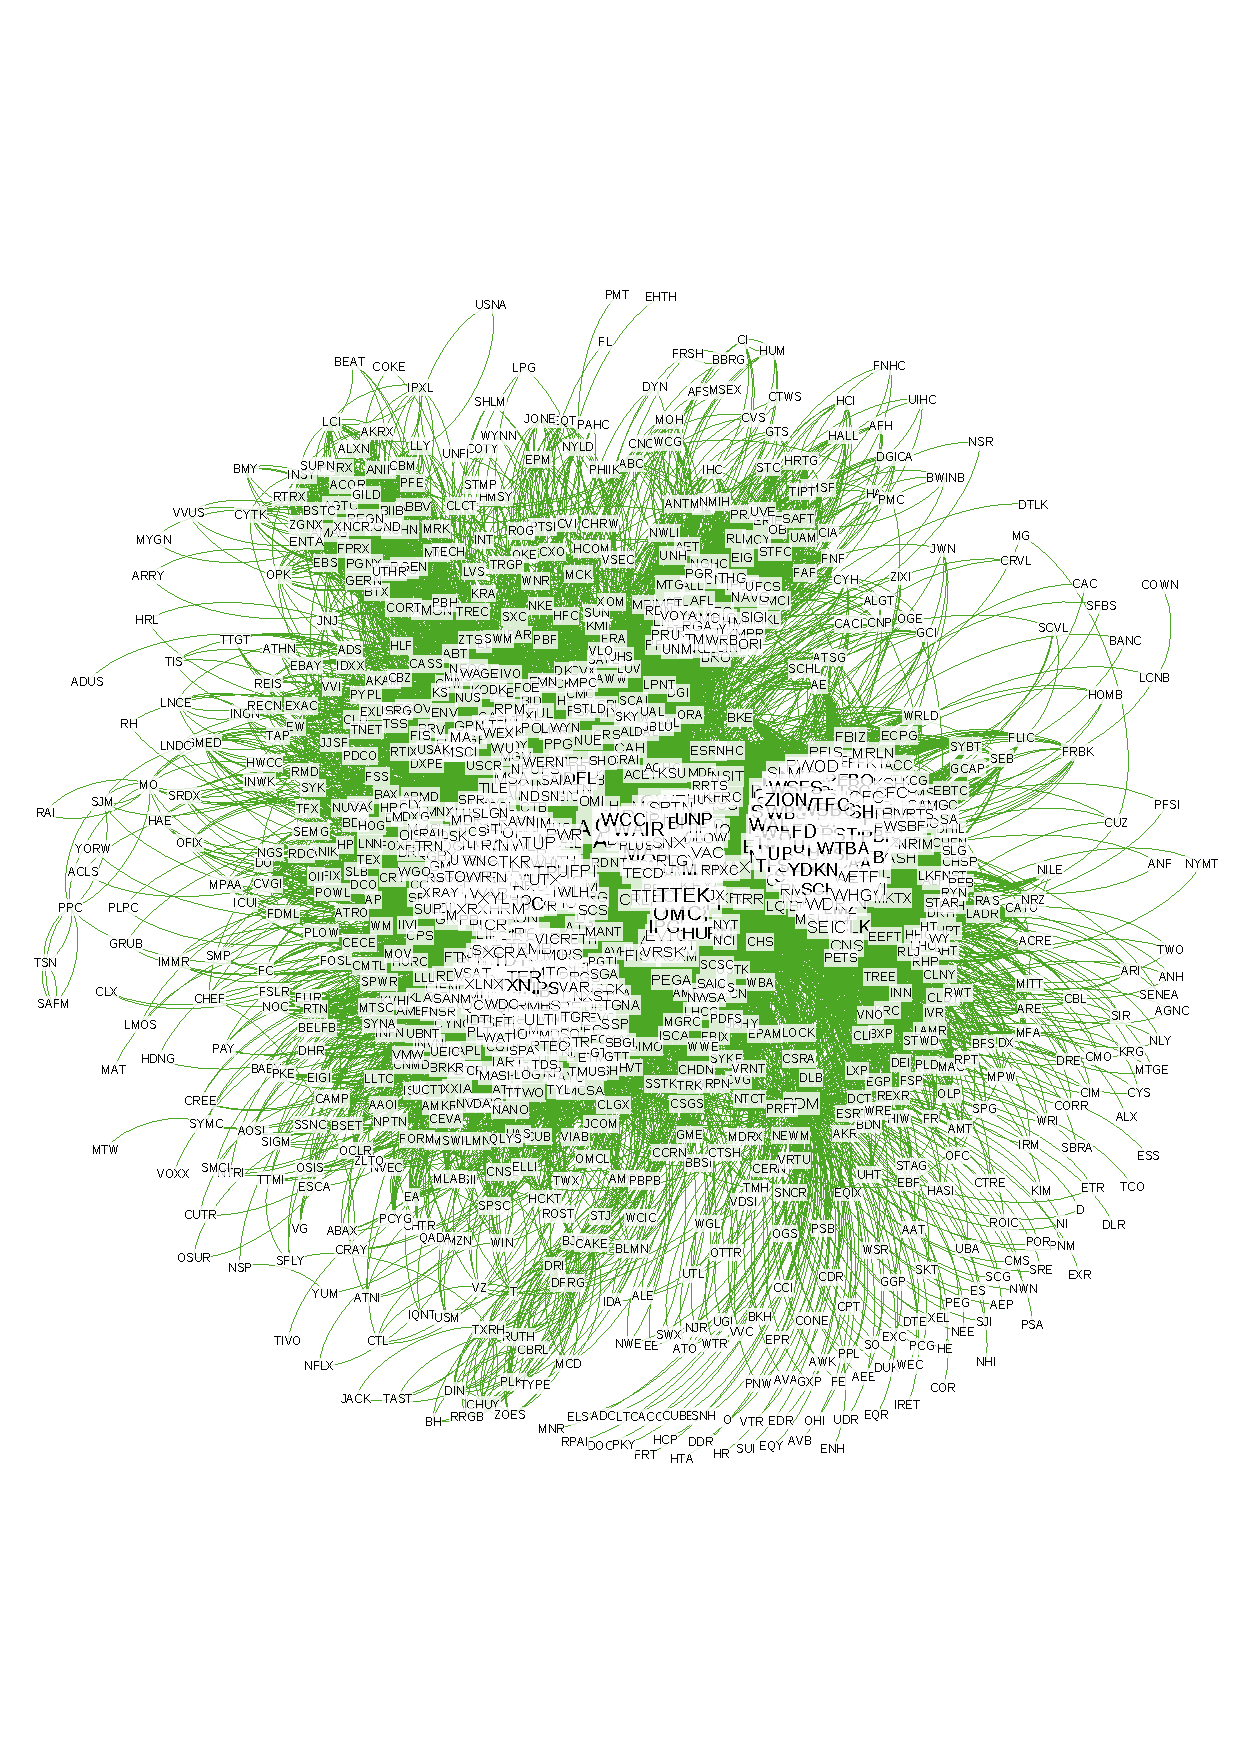
\includegraphics[width=14cm]{Graph_01}
	\end{center}
	\caption{Transaction densities}
	\label{fig:Graph_01}
\end{figure}


It is obvious that the larger values assigned to $\theta_{EIO}$ and $\theta_{corr}$, the more significant for the weights and directions of the remaining edges. But if the network is too sparse, it can not be strongly or weakly connected hence the network becomes inefficient. As a result, this paper selects the threshold-value-pair $\theta_{EIO}=0.292$ and $\theta_{corr}=0.379$ to construct directed unweighted stock network and directed weighted stock network.

%这里放Gephi的图片 可以随机选择一半的结点作为生成

\section{Analysis of the directed unweighted network}
% 对幂指数分布的统计检验
A directed Watts Strogatz small-world network and a random network with the same number of nodes and edges with the stock directed unweighted network are generated. Table~\ref{tab:three} compares the main topologies of the three different networks.

\begin{table}
	\begin{center}
		\begin{tabular}{|r|c|c|c|}\hline\hline
			Directed networks&Stock network&Small-world network&Random network\\\hline
			Number of nodes&1418&1418&1418\\
			Number of edges&102051&102088&102097\\
			Out-degree distribution&Power-law&Normal&Normal\\
			Average out-degrees&143.94&143.99&144.00\\
			Average path length&2.775&2.005&1.973\\
			Clustering coefficient&0.4675&0.1367&0.05105\\
			Global efficiency&0.2563&0.5161&0.5216\\
			Local efficiency&0.6276&0.5027&0.4456\\
			Assortativity&0.02004&-0.002180&0.001452\\
			\hline\hline
		\end{tabular}
	\end{center}
	\caption{Main properties of stock network, small-world network, and random network}\label{tab:three}
\end{table}

\subsection{Power-law distribution}
According to the table~\ref{tab:three}, the values of average out-degrees of stock network, small-world network and random network are almost the same due to the similar number of nodes and edges, but in terms of the distributions of out-degrees, stock network is different from the others. 

Figure~\ref{fig:distributionsm} and \ref{fig:distributionrd} show clearly that the out-degree distribution of small-world network and random network follow the normal distribution, i.e, most degree numbers of nodes fall in the middle range, while figure~\ref{fig:G_out_degree_distribution_square} illustrates that for the stock network, only a few number of nodes show higher out-degree, while most nodes are in the positions of low out-degree level. The distribution of the directed stock price return networks follows power-law distribution with the exponent of 4.057.

%Power-law distribution reveals that most of the nodes have a small degree while a few modes have a higher degree.
\subsection{Small-world property}
The average path length of small-world network and random network are both close to 2, indicates that taking any node in the network, it can expect to reach any other nodes just through one node as medium. For stock network, the expectation number of medium nodes is 1.775, which is also a small number for connection, so like small-world and random networks, stock network also has the small-world property.

% Efficiency.
\subsection{Community feature}
The larger value of clustering coefficient for stock network than the other two networks indicating that the nodes in stock network tend to cluster together. Therefore, communities of stock network will be identified implementing the community detection algorithm for directed networks in this section. According to the industrial sectors to which most component stocks are belong, as figure~\ref{fig:community_sector_stacked} shows, following five communities are identified: (1) Production (2) Finance (3) Livelihood (4) Insurance and chemical products (5) Utilities and financial vehicles.

It can see from figure~\ref{fig:community_graph} that the community of finance (green) has a very dense structure, connected closely inside and completely exclusive from other communities. The communities of production (purple) and livelihood (blue) are sparsely distributed while there are some large-sized nodes acting as hubs of the overall network. The other two communities are more interesting because they have peculiar structures.

Every industrial sectors of individual stocks in community are identified to investigate the properties of the community of insurance and chemical products (yellow). As figure~\ref{fig:community_4} illustrates and through the investigation, most firms in the upper and lower clusters are in the sectors of "chemical products" and "Insurance carriers and related activities" respectively, while firms between the two big clusters, like "MCK" (McKesson) and "CAH" (Cardinal Health), are large medical supplier, pharmaceutical and heathcare service companies with high out-degrees to both of the two clusters. Apart from that, there are also considerable number of links from the upper cluster to the hubs of chemical companies. Thus, it is reasonable to infer that the prices of medicines have significant influence to medical insurance industry, additionally the purchases of chemical products of pharmaceutical firms and the sales of chemical products have made pharmaceutical and chemical companies influence to each other.

Another investigation towards the community of utilities and financial vehicles (orange) is conducted by the same measure. As figure~\ref{fig:community_5} illustrates, there is one huge hub (PDM) which is the company "Piedmont Office Realty Trust" among the community while all the others are one-degree nodes located remotely. More links from the hub to the rest than the opposite direction, and also the weights of the former links are generally higher. The hub, "Piedmont Office Realty Trust", is a real estate investment trust company, and the rest in the community contains 59 "Funds, trusts, and other financial vehicles" firms and 44 "Utilities" firms. % infer

Although the assortativity values for the three networks are all non-significant, 

\begin{figure}
	\begin{center}
		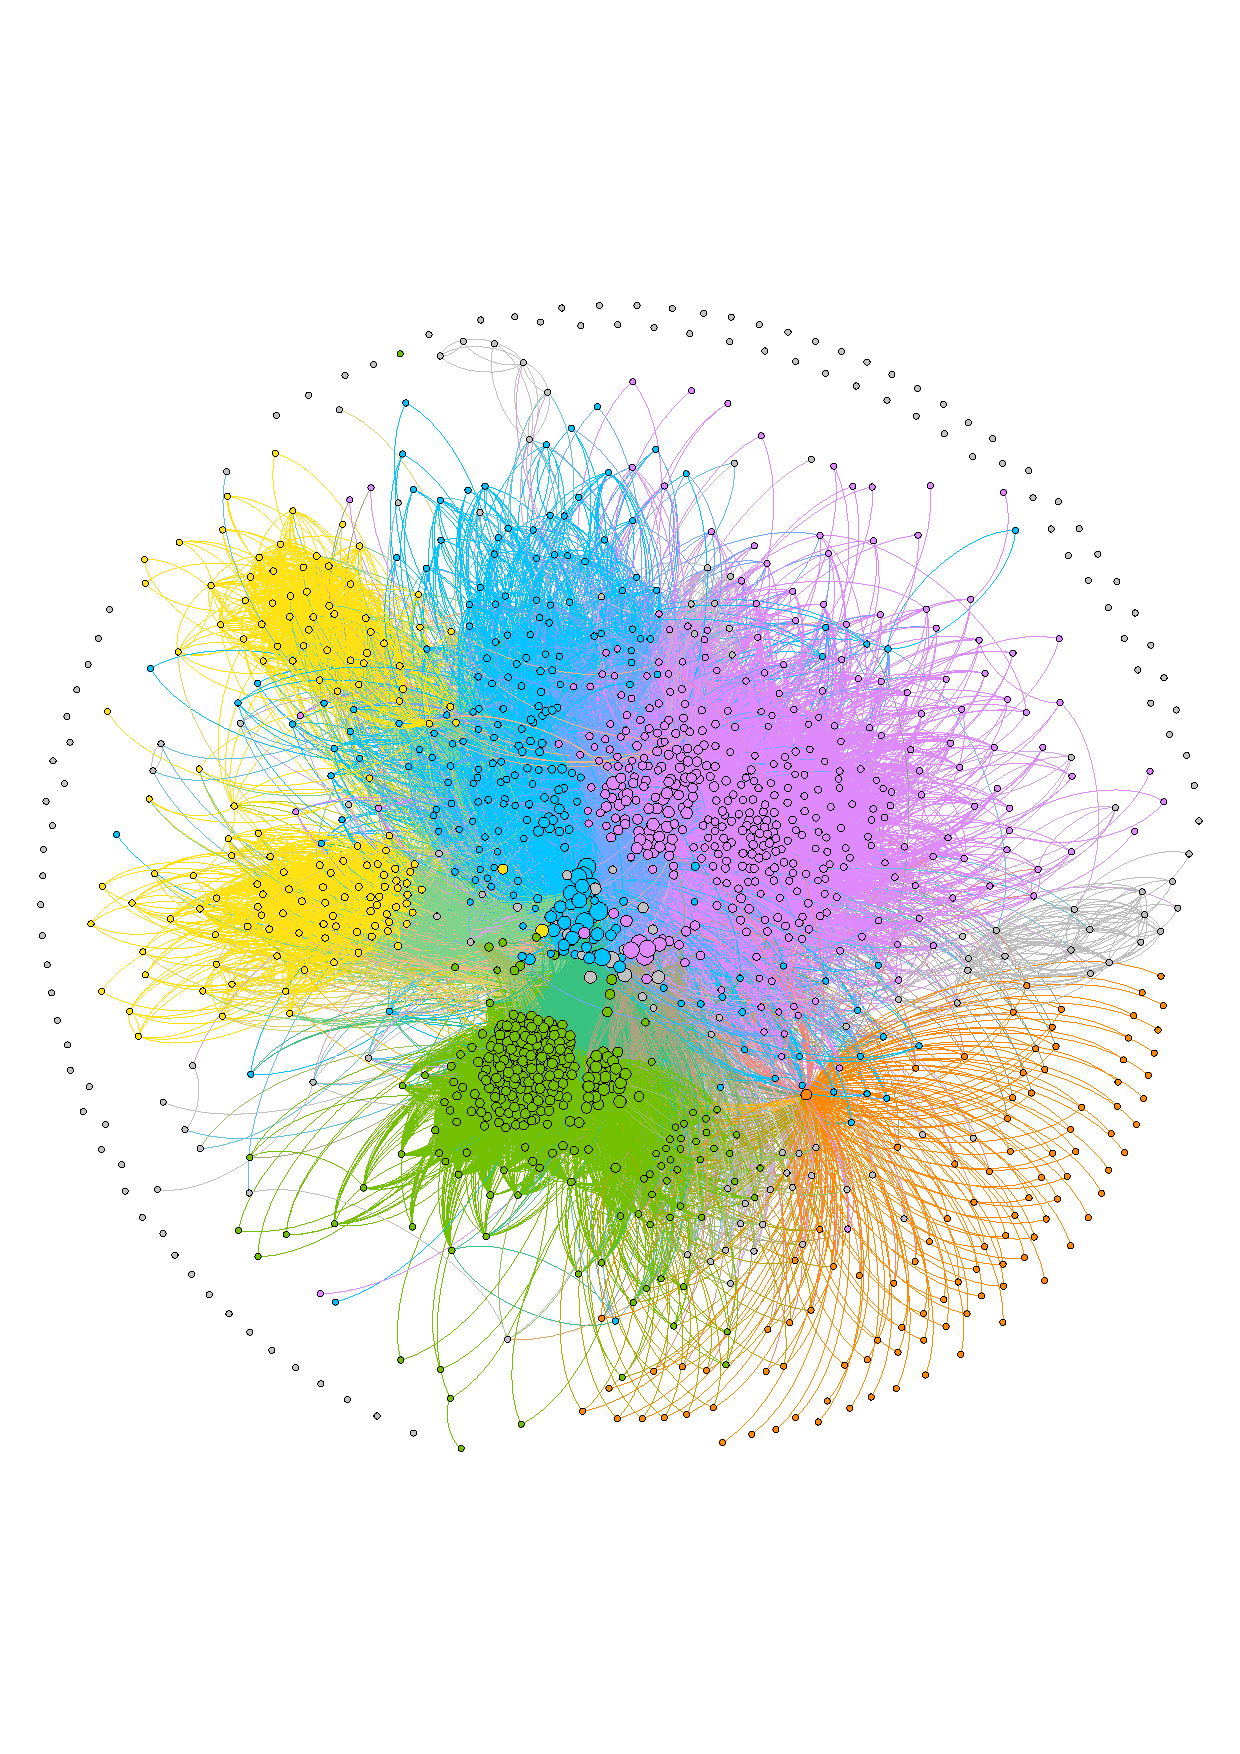
\includegraphics[width=14cm]{community_graph}
	\end{center}
	\caption{Community structure of the 2016 US stock price return network. Five distinct communities are detected represented by different colours of nodes. The direction of edge is  clockwise. The size of nodes and thickness of edges are related to the value of degrees and weights. The grey nodes do not belong to any communities and most of them have zero degree.}
	\label{fig:community_graph}
\end{figure}

\begin{figure} % 各个单独的群落
	\subfloat[Production]{%
		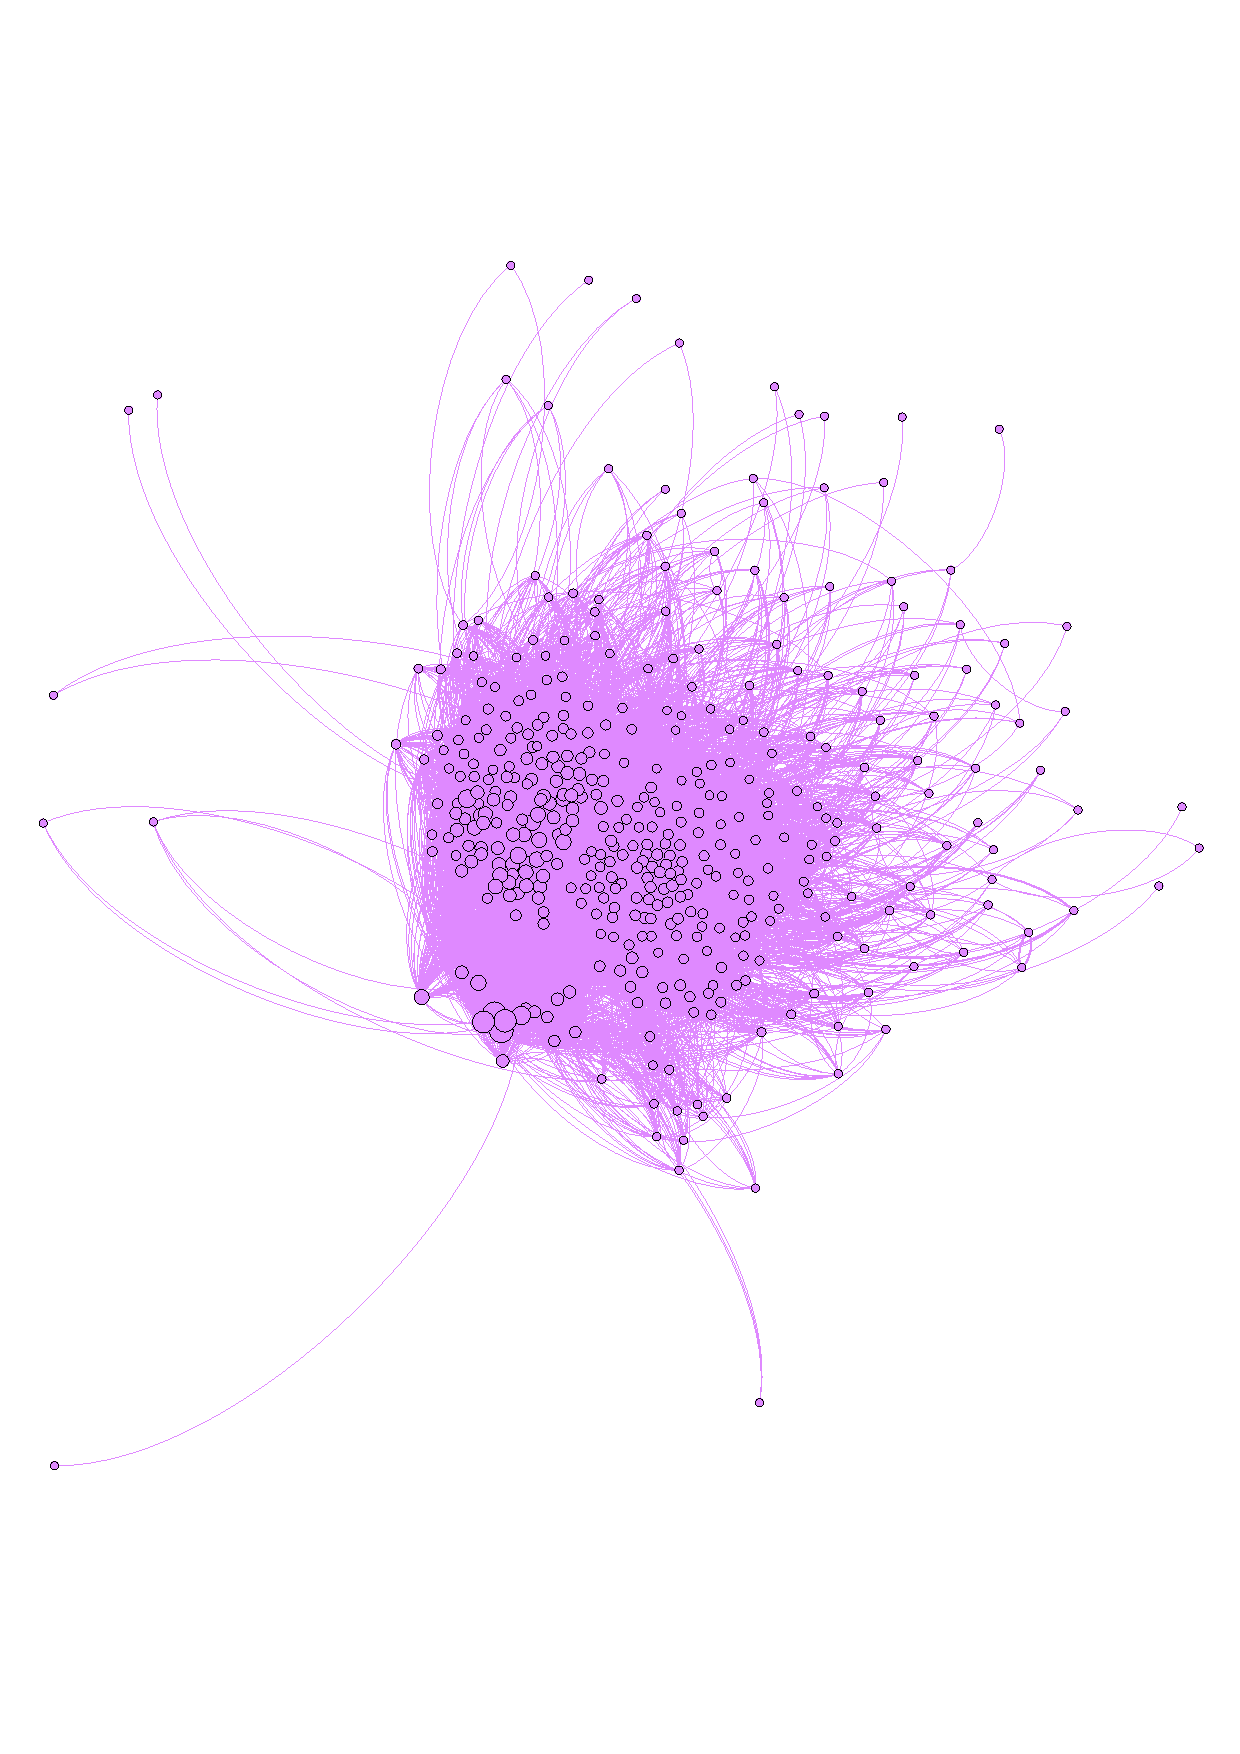
\includegraphics[width=0.46\textwidth]{community_1}%
		\label{fig:community_1}%
	}%
	\hfill%
	\subfloat[Finance]{%
		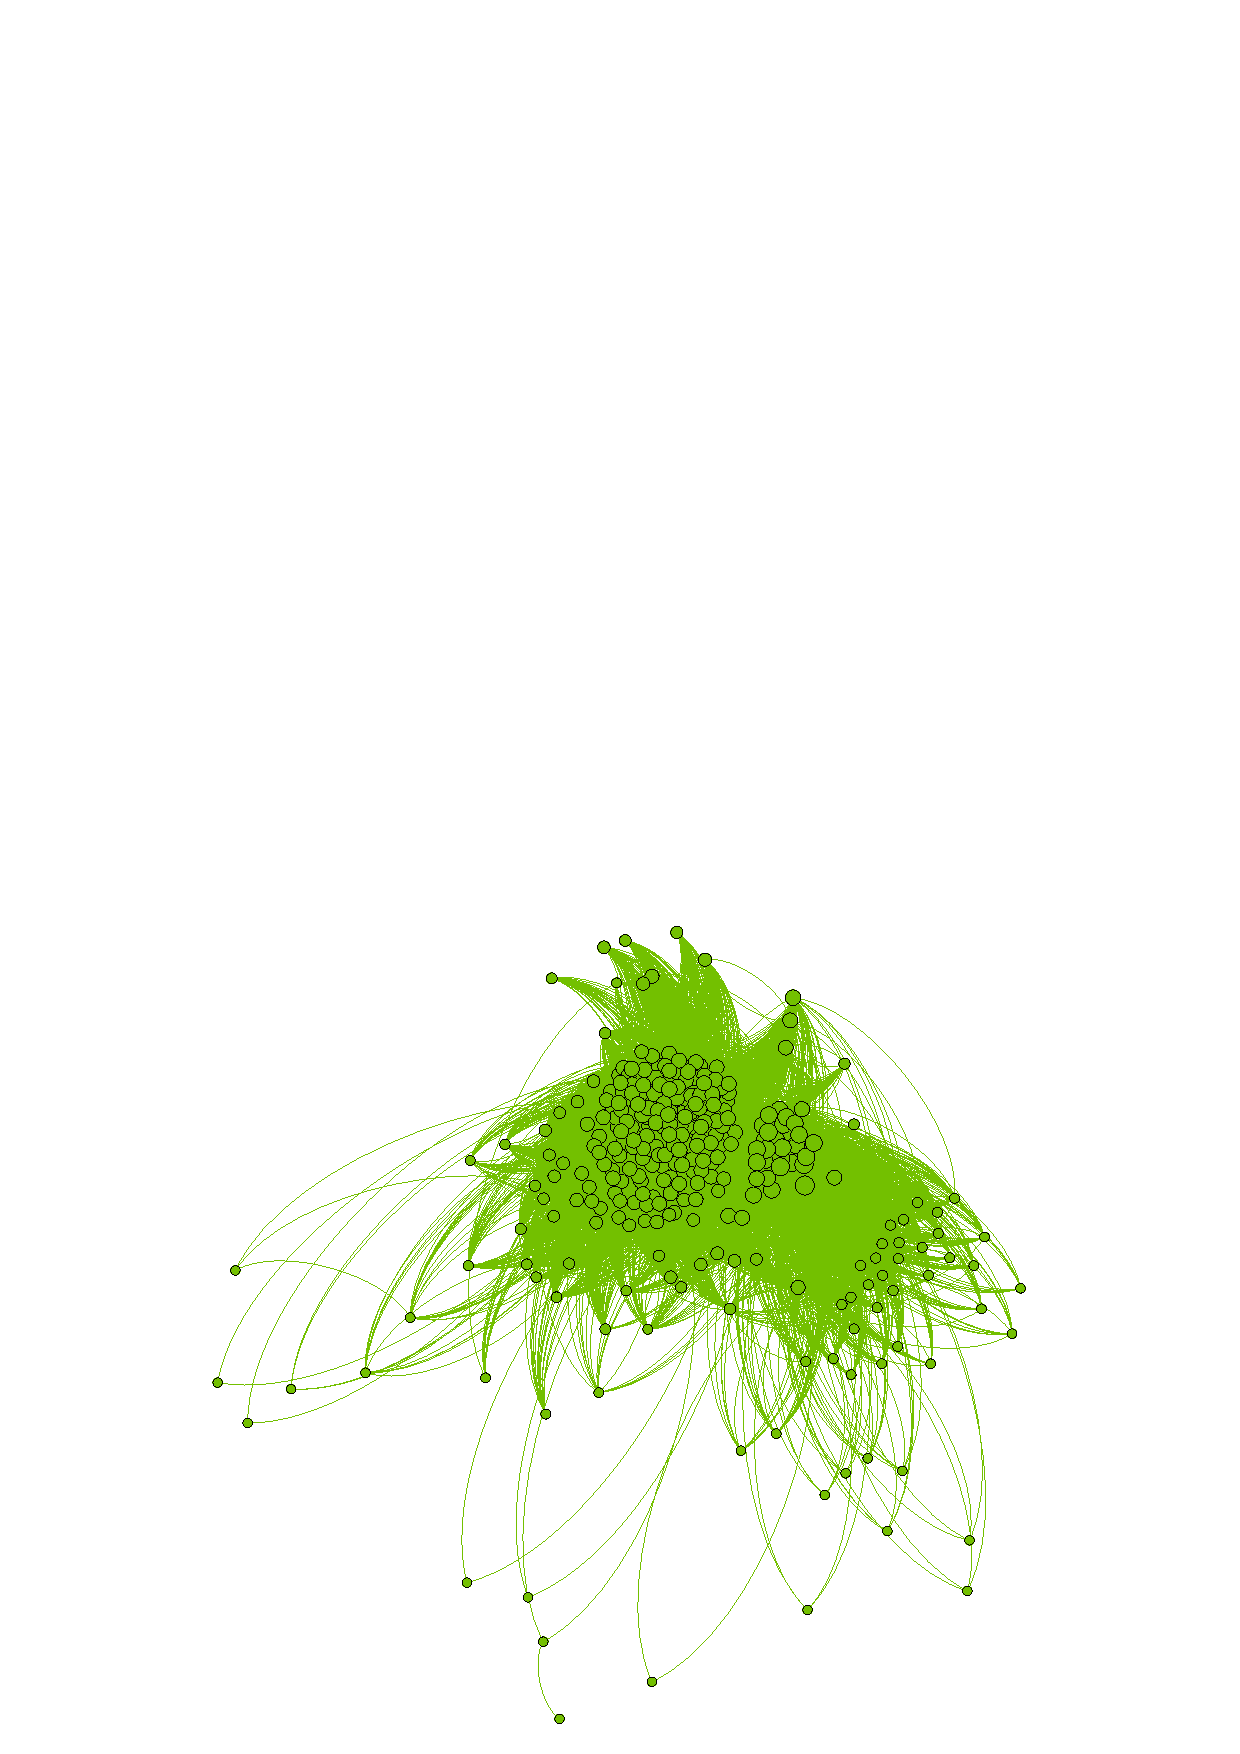
\includegraphics[width=0.46\textwidth]{community_2}%
		\label{fig:community_2}%
	}%
	\hfill%
	\subfloat[Livelihood]{%
		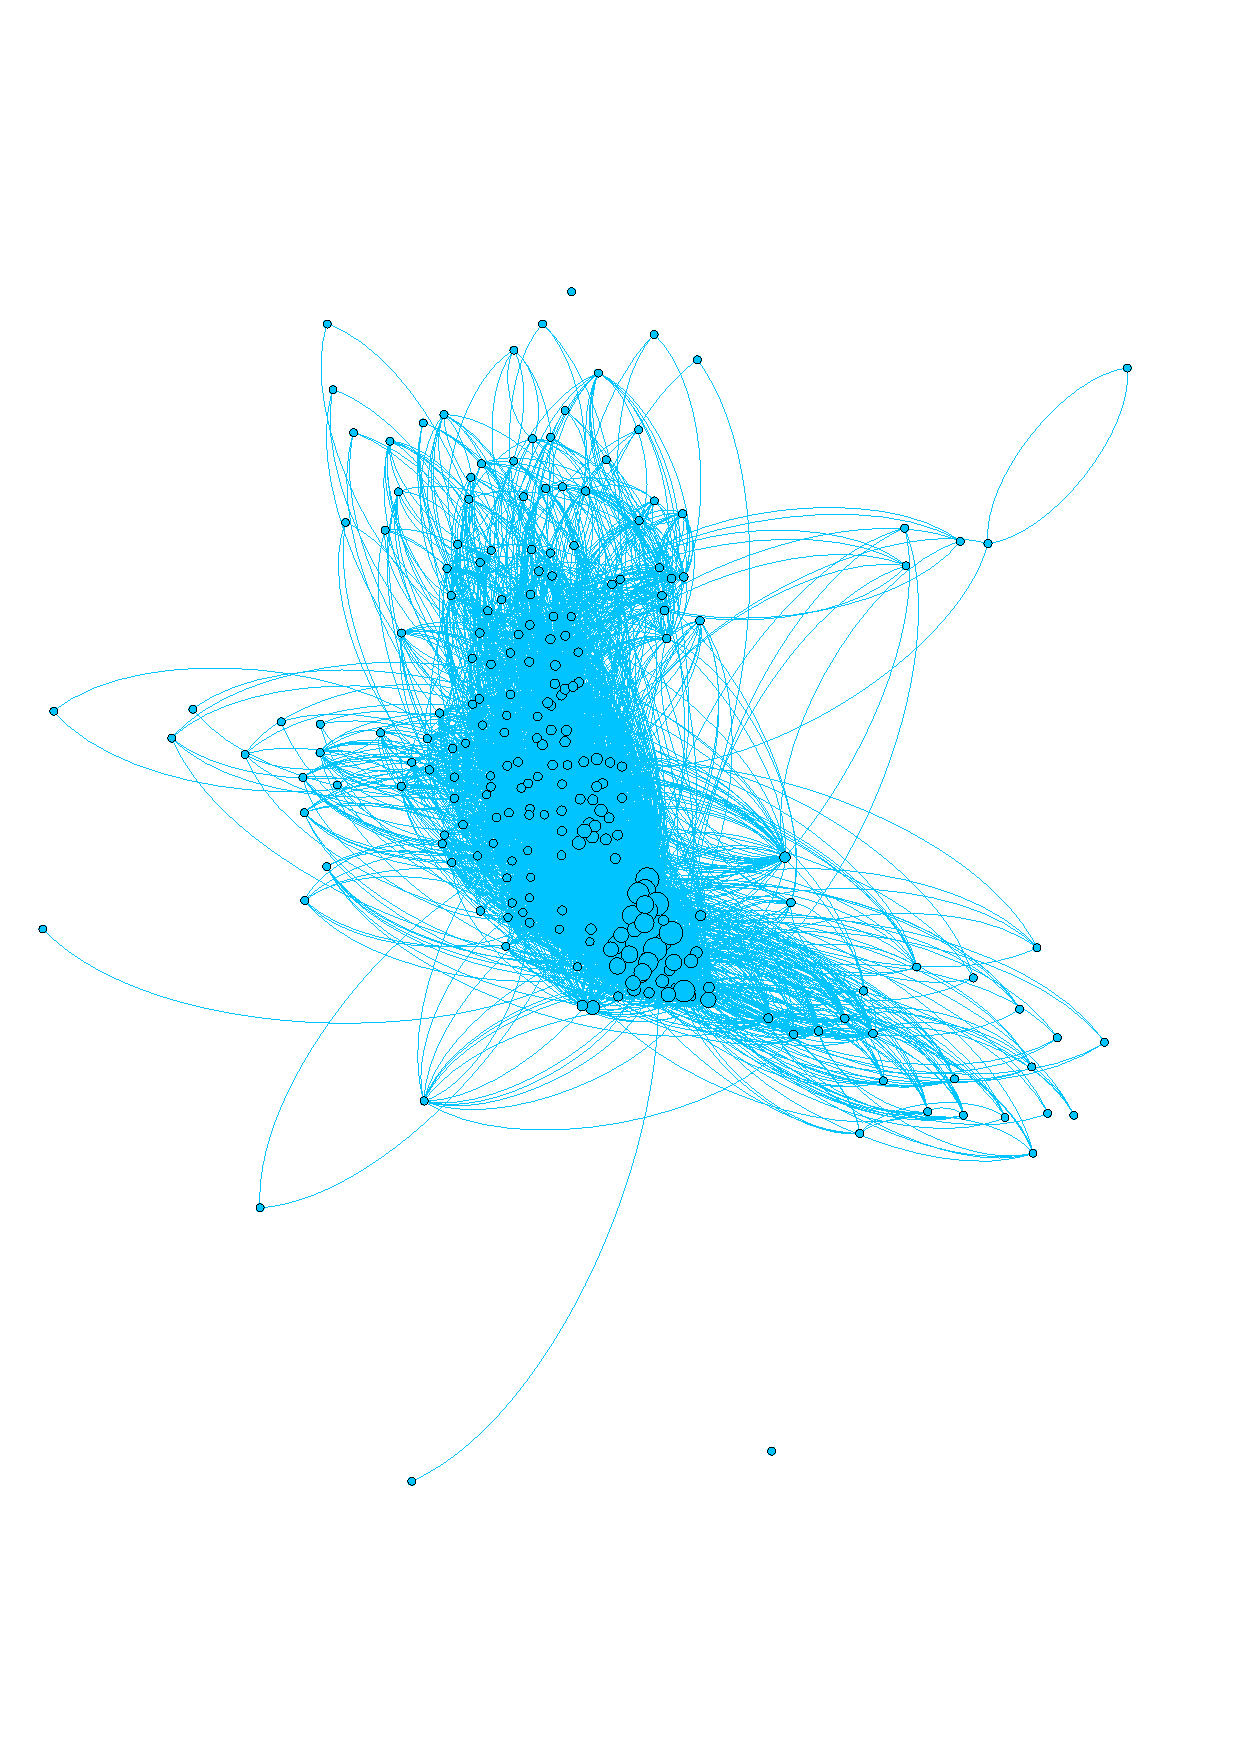
\includegraphics[width=0.46\textwidth]{community_3}%
		\label{fig:community_3}%
	}%
	\hfill%
	\subfloat[Insurance and chemical products]{%
		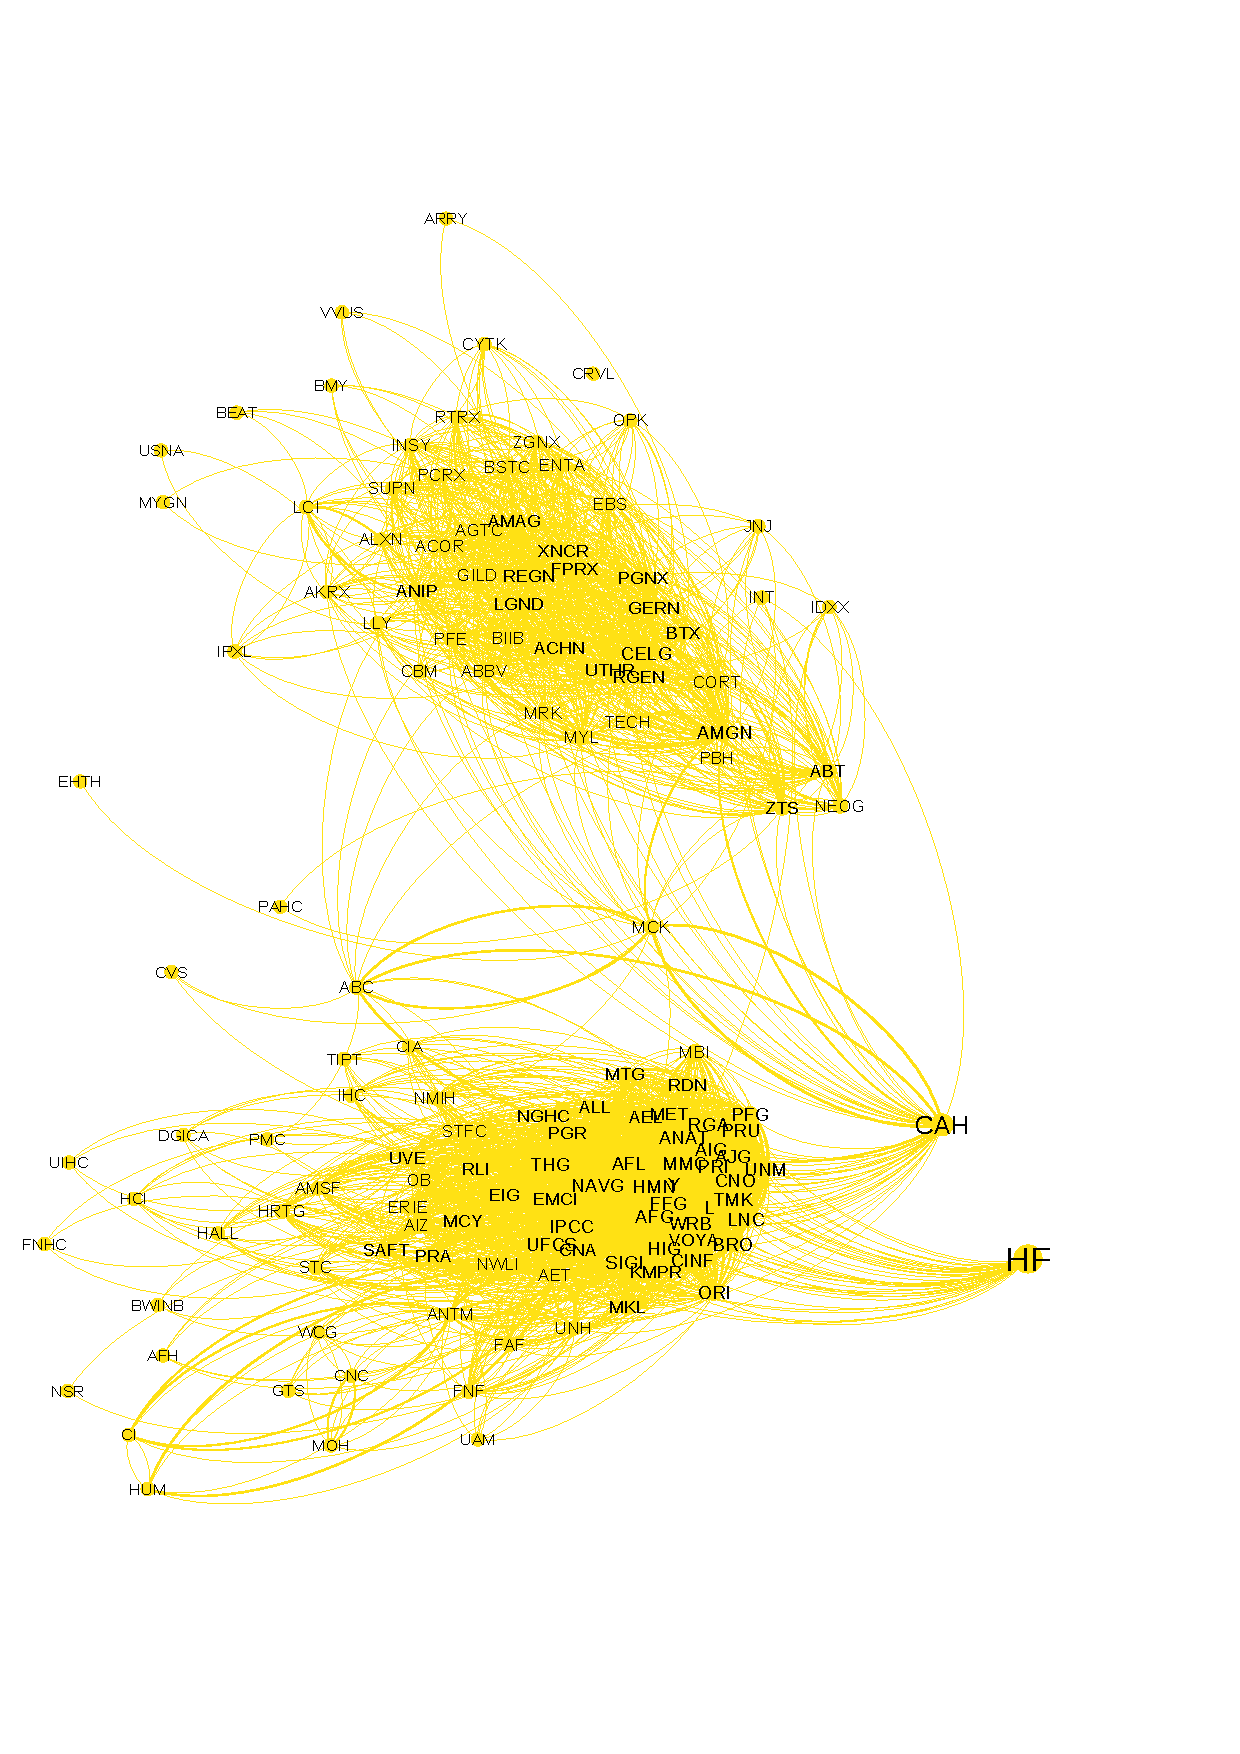
\includegraphics[width=0.46\textwidth]{community_4}%
		\label{fig:community_4}%
	}%
	\hfill%
	\subfloat[Utilities and financial vehicles]{%
		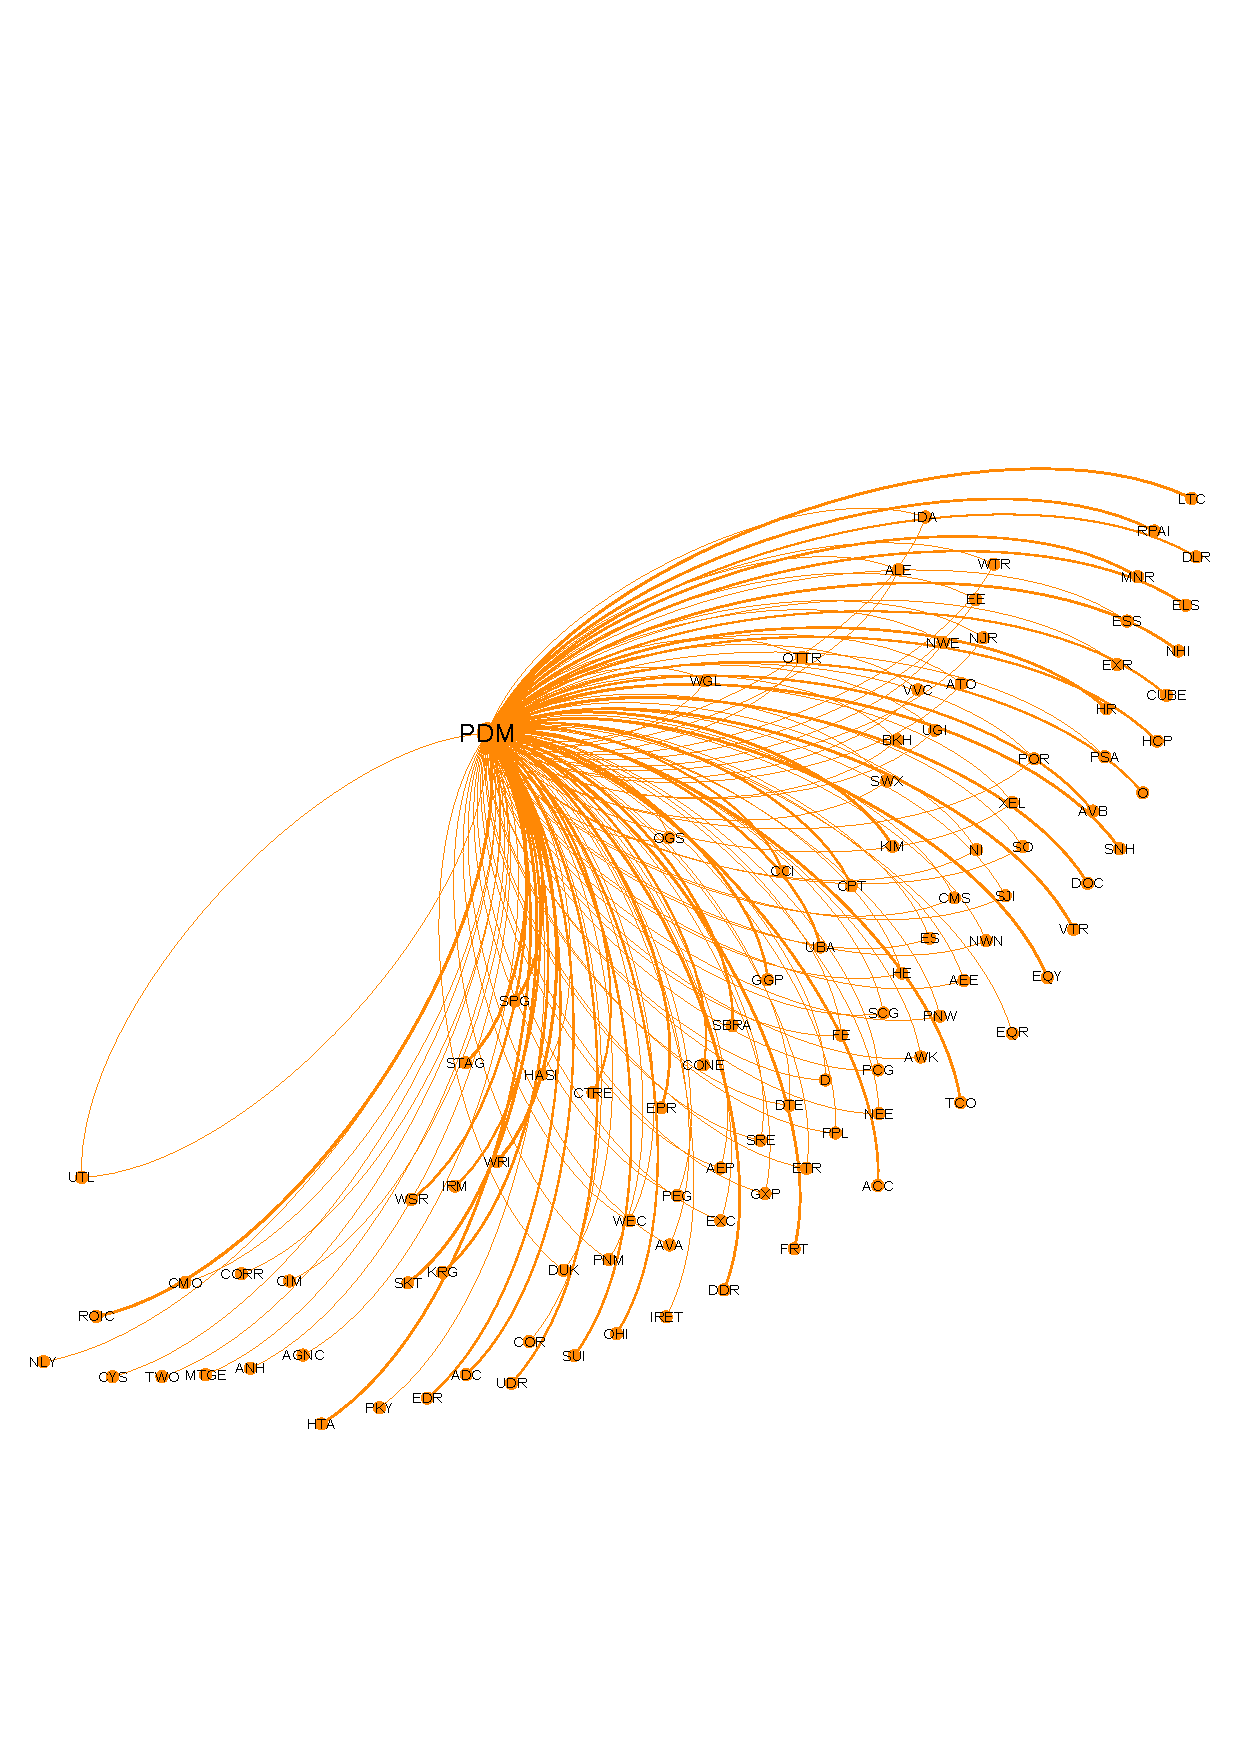
\includegraphics[width=0.46\textwidth]{community_5}%
		\label{fig:community_5}%
	}%
	\caption{Solely community views of the directed stock network. Stock tickers are displayed for the sparsely distributed communities.} \label{fig:distinctcommunities}
\end{figure}

\begin{figure} % 群落的行业柱形图
	\begin{center}
		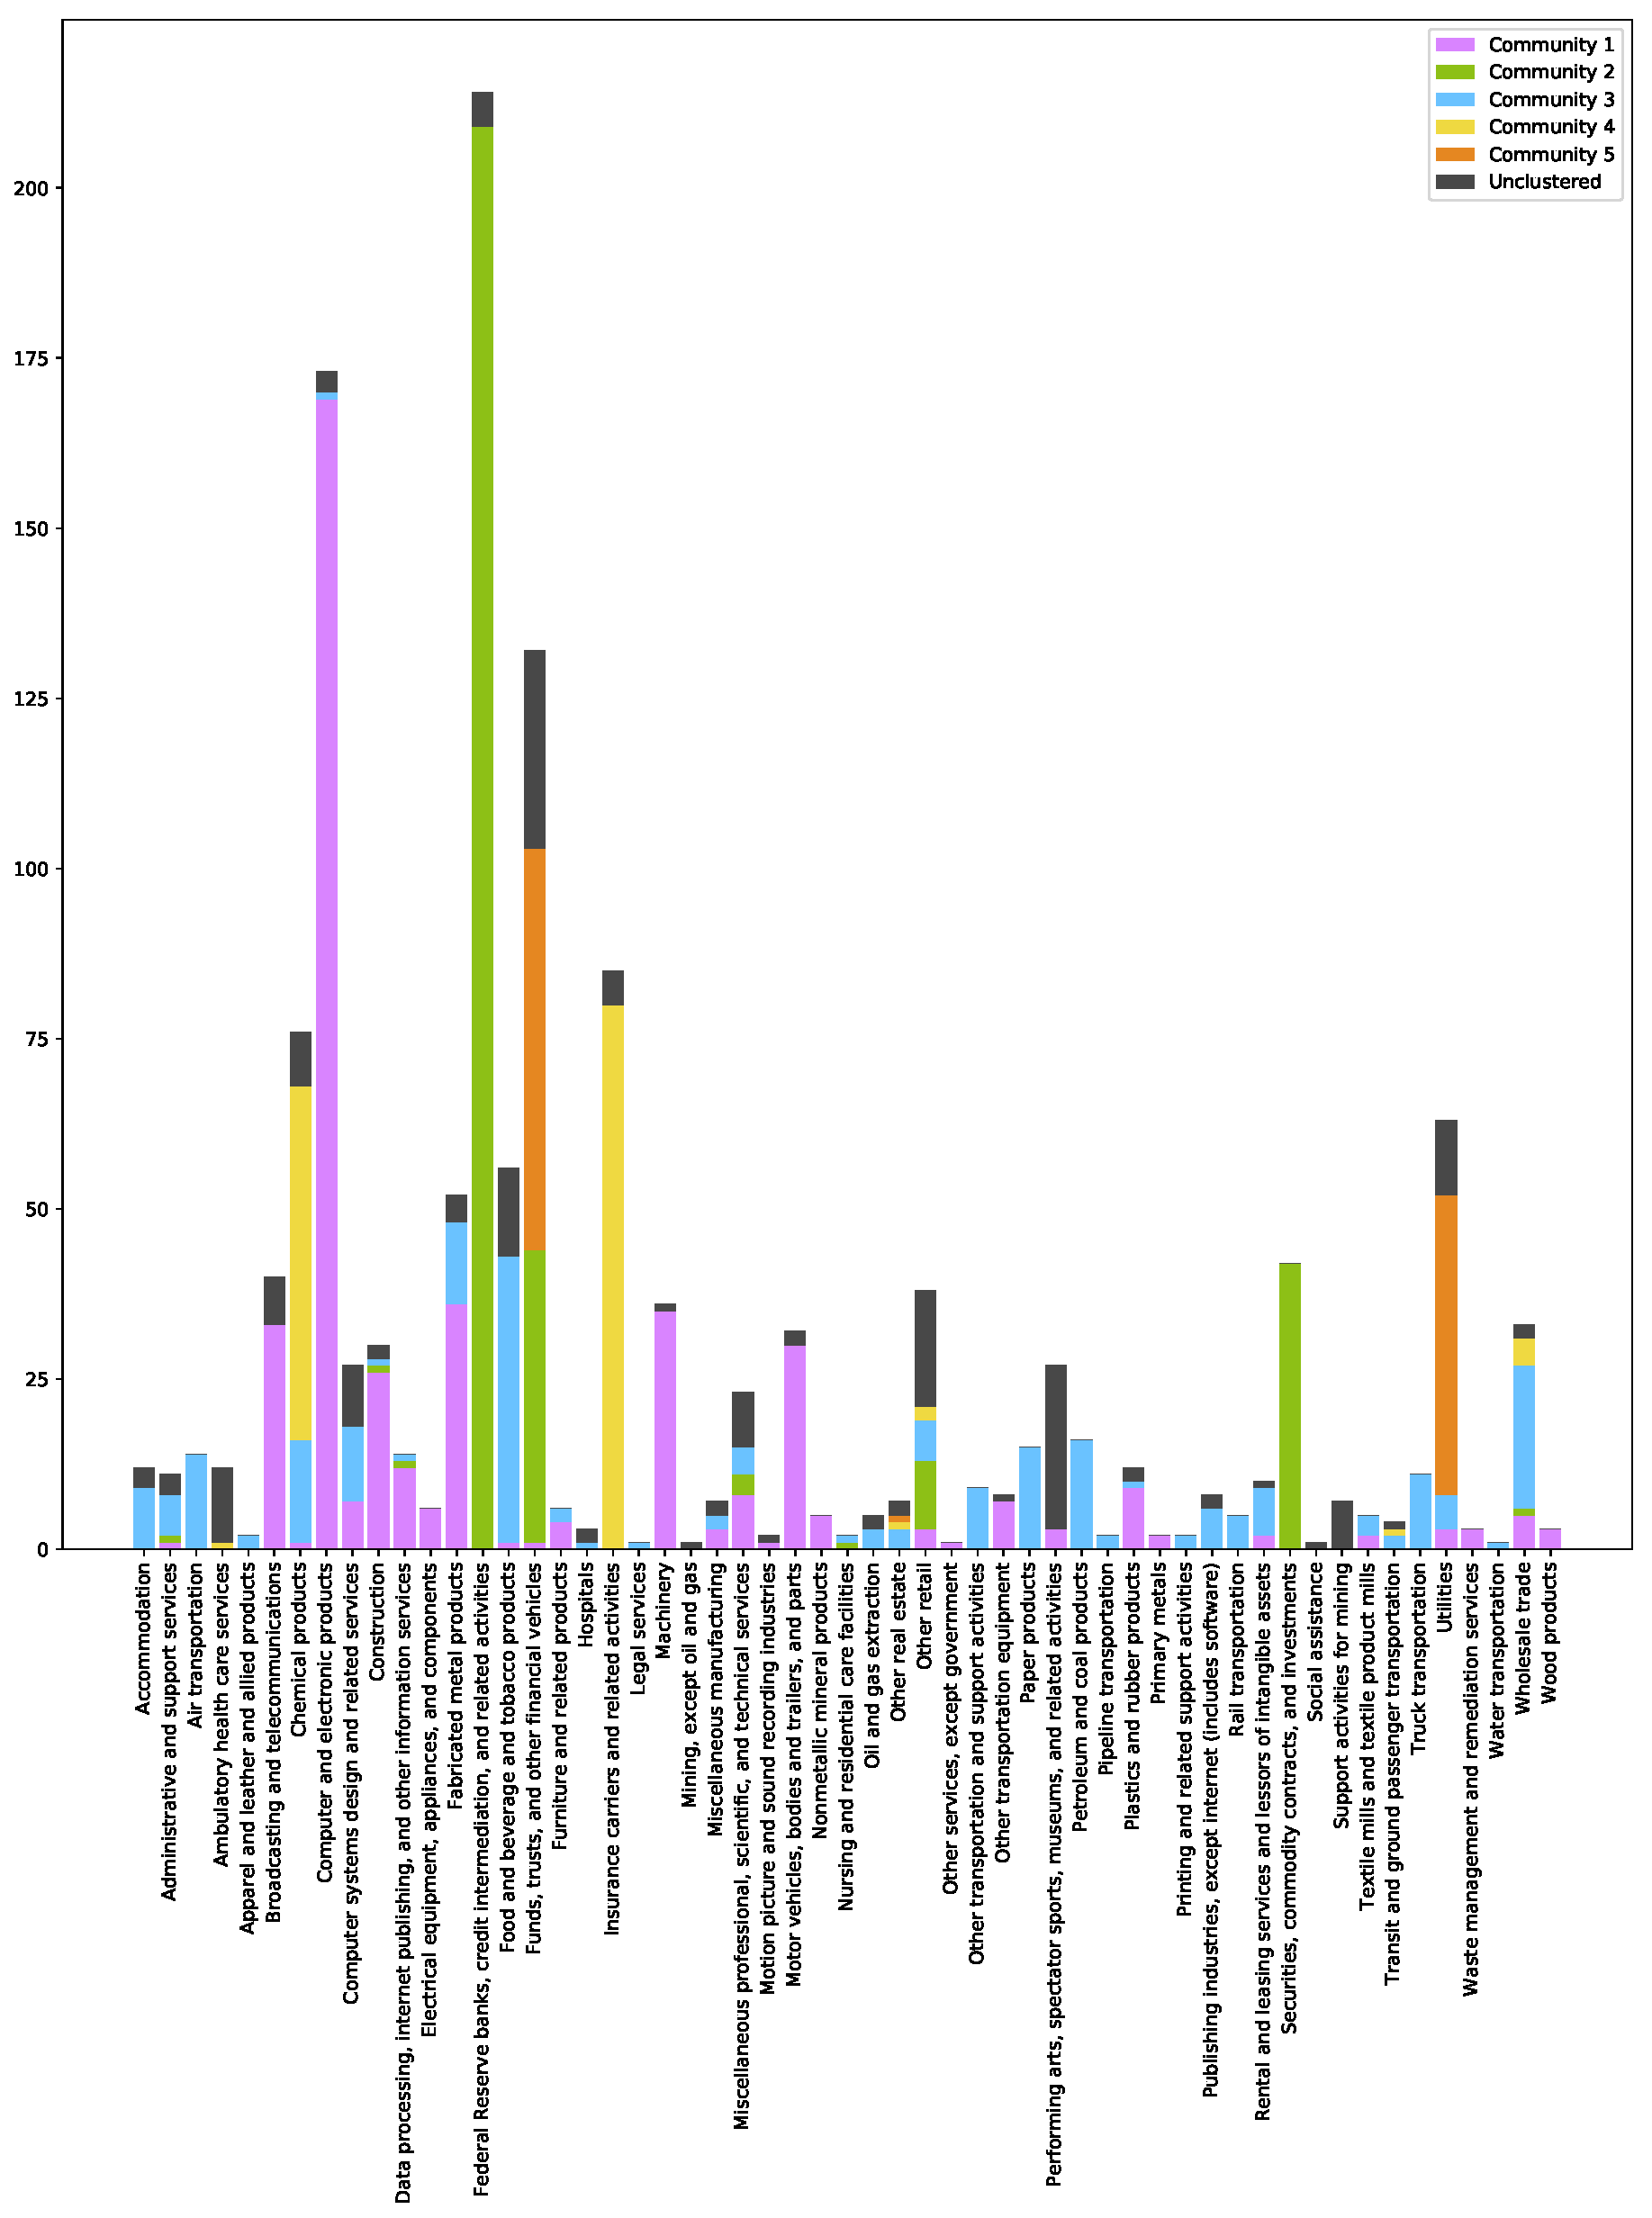
\includegraphics[width=14cm]{community_sector_stacked}
	\end{center}
	\caption{Count of stocks of each communities by industrial sectors. Sectors are arranged alphabetically.}
	\label{fig:community_sector_stacked}
\end{figure}

\begin{table}
	\begin{center}
		\begin{tabular}{|r|c|}\hline\hline
			&Undirected stock network\\\hline
			Degree distribution&Power-law\\
			Average out-degrees&Power-law\\
			Average path length&2.775\\
			Clustering coefficient&0.4675\\
			Global efficiency&0.2563\\
			Local efficiency&0.6276\\
			Assortativity&0.02004\\
			\hline\hline
		\end{tabular}
	\end{center}
	\caption{Main topologies of conventional stock price network}\label{tab:conventional}
\end{table}

\begin{figure}
	\subfloat[Empirical out-degree distribution]{%
		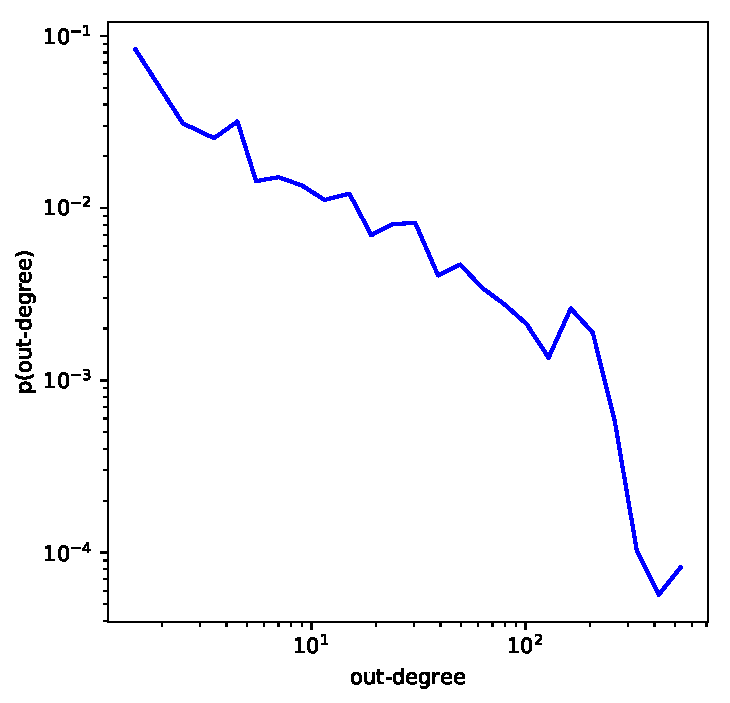
\includegraphics[width=0.46\textwidth]{G_out_degree_distribution_square}%
		\label{fig:G_out_degree_distribution_square}%
	}%
	\hfill%
	\subfloat[CCDF and power-law fit]{%
		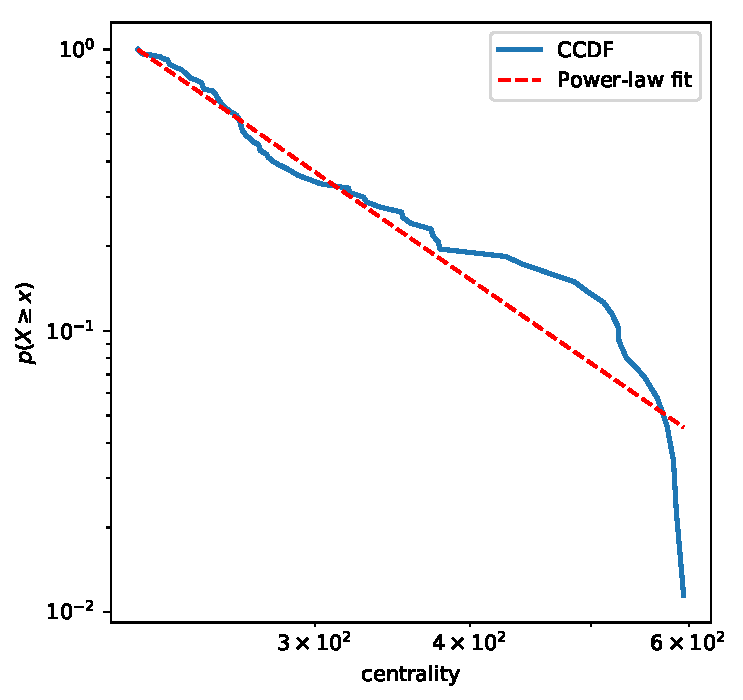
\includegraphics[width=0.465\textwidth]{out_degree_log_fit_square}%
		\label{fig:out_degree_log_fit_square}%
	}%
	\caption{Out-degree distribution of stock network} \label{fig:outdegreedistribution}
\end{figure}

\begin{figure} % P-P SW
	\centering
	\subfloat[Empirical out-degree distribution]{
		\label{subfig:G_sw_out_degree_distribution}
		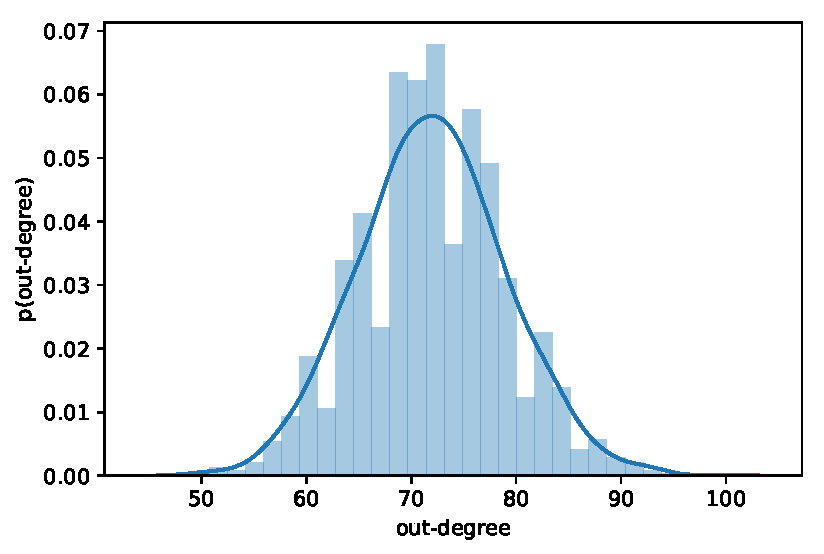
\includegraphics[width=12cm]{G_sw_out_degree_distribution} }
	
	\subfloat[P-P plot]{
		\label{subfig:G_ws_mat_prob_plot}
		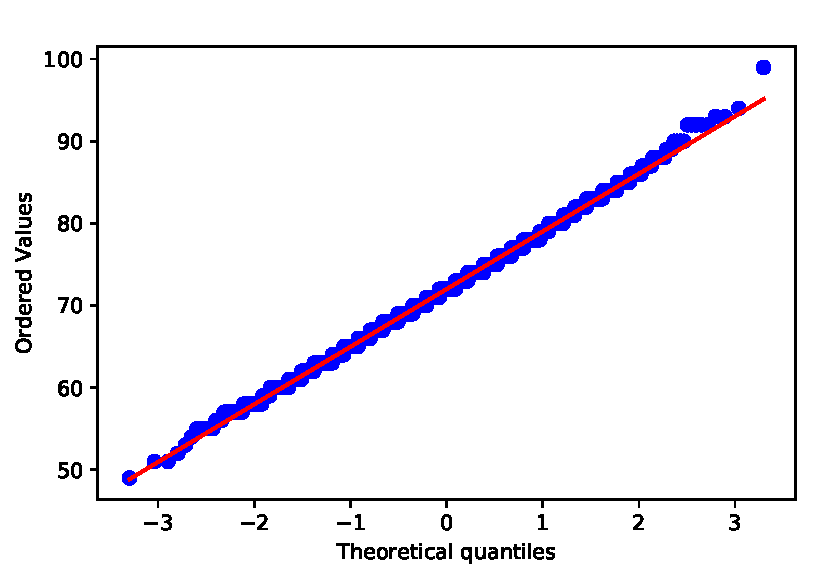
\includegraphics[width=12cm]{G_ws_mat_prob_plot} }
	
	\caption{Out-degree distribution and P-P plot of small-world network}
	\label{fig:distributionsm}
\end{figure}

\begin{figure} % P-P rd
	\centering
	\subfloat[Empirical out-degree distribution]{
		\label{subfig:G_rd_out_degree_distribution}
		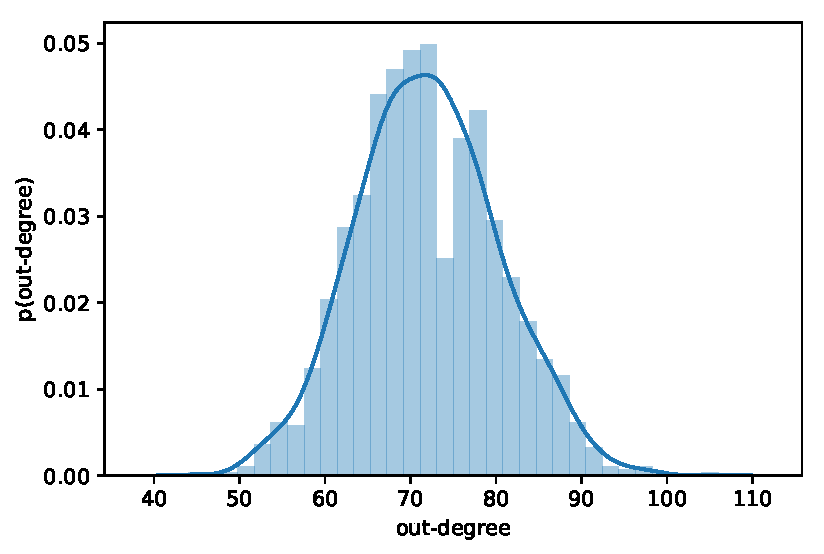
\includegraphics[width=12cm]{G_rd_out_degree_distribution} }
	
	\subfloat[P-P plot]{
		\label{subfig:G_rd_prob_plot}
		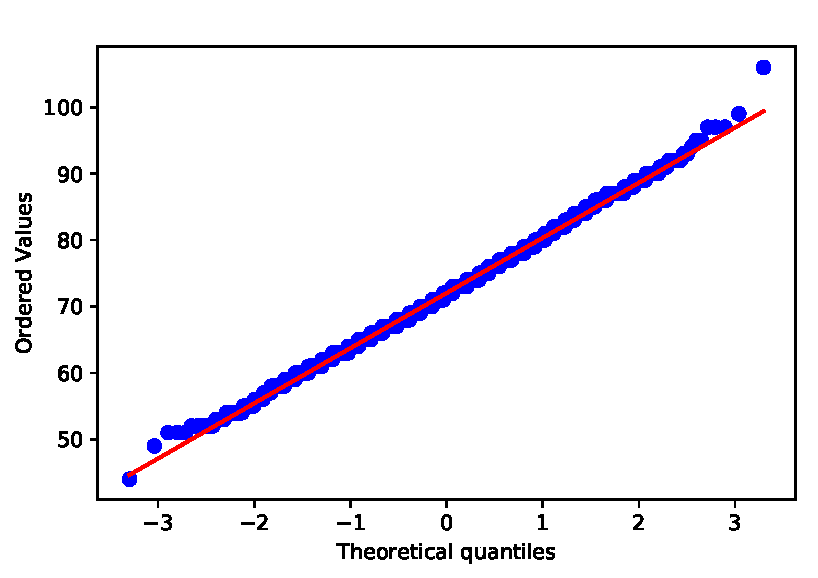
\includegraphics[width=12cm]{G_rd_prob_plot} }
	
	\caption{Out-degree distribution and P-P plot of random network}
	\label{fig:distributionrd}
\end{figure}


\iffalse
\begin{figure}
	\begin{center}
		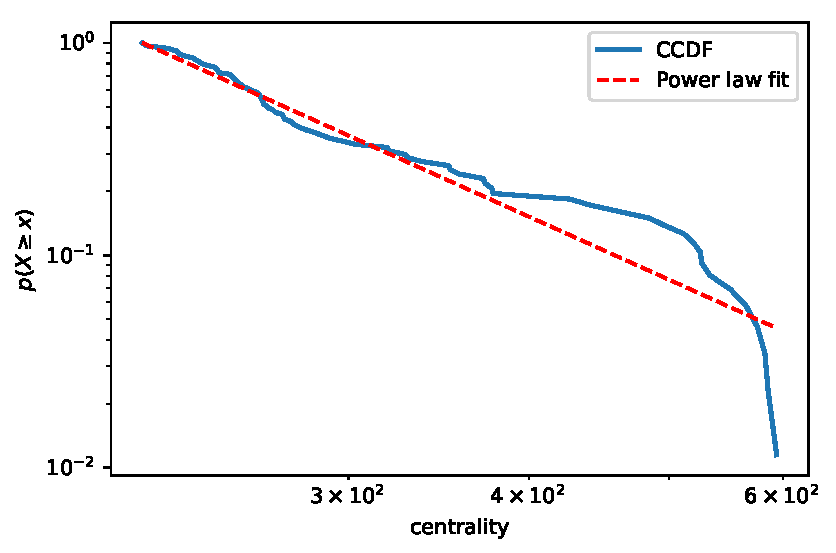
\includegraphics[width=15cm]{out_degree_log_fit}
	\end{center}
	\caption{Amounts of edges per EIO-threshold and correlation-coefficient-threshold}
	\label{fig:out_degree_log_fit}
\end{figure}
\fi

%Clustering coefficient
%行业内非对称边和行业间对称边的数量
%Global/ local efficiency

%Betweenness centrality

%Community detection


\section{Analysis of the directed weighted network}
% Strength distribution
\begin{table}
	\begin{center}
		\begin{tabular}{|r|c|}\hline\hline
			&Undirected stock network\\\hline
			Strength distribution&Power-law\\
			Average centrality&1\\
			Weighted assortativity&0.1244\\
			\hline\hline
		\end{tabular}
	\end{center}
	\caption{Main topologies of directed weighted stock price network}\label{tab:weighted}
\end{table}

\begin{figure} % P-P sw
	\centering
	\subfloat[Bivariate distribution of cumulative sum of daily return]{
		\label{subfig:sum_return_centrality}
		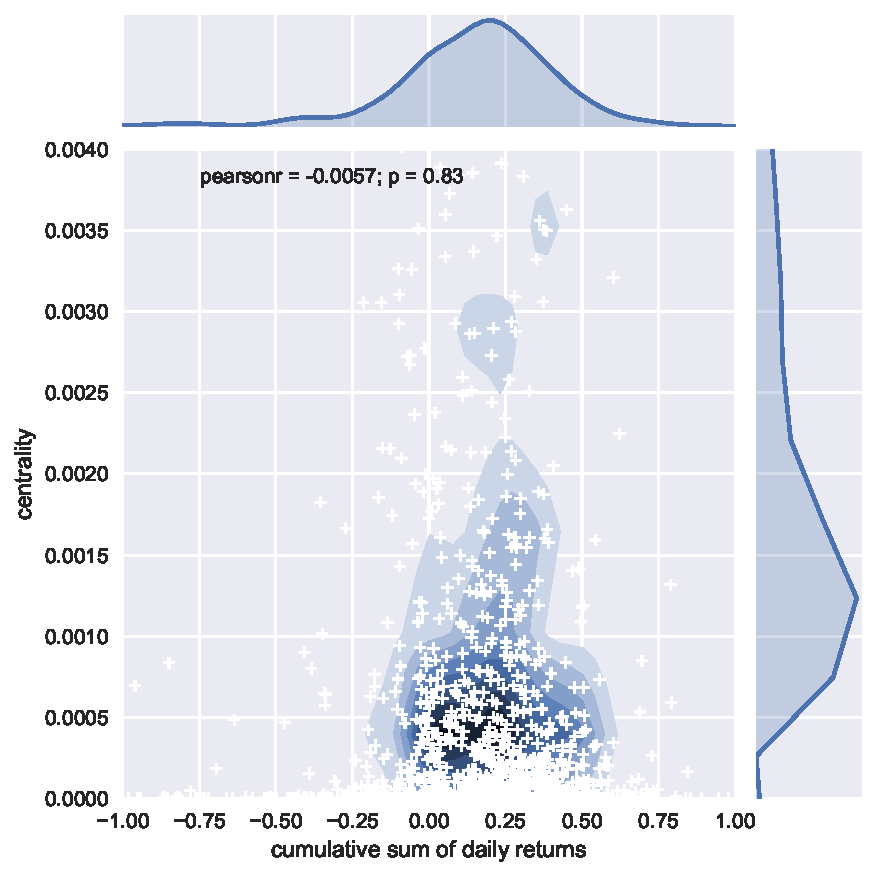
\includegraphics[width=10cm]{sum_return_centrality} }
	
	\subfloat[Bivariate distribution of standard deviation of daily return]{
		\label{subfig:std_return_centrality}
		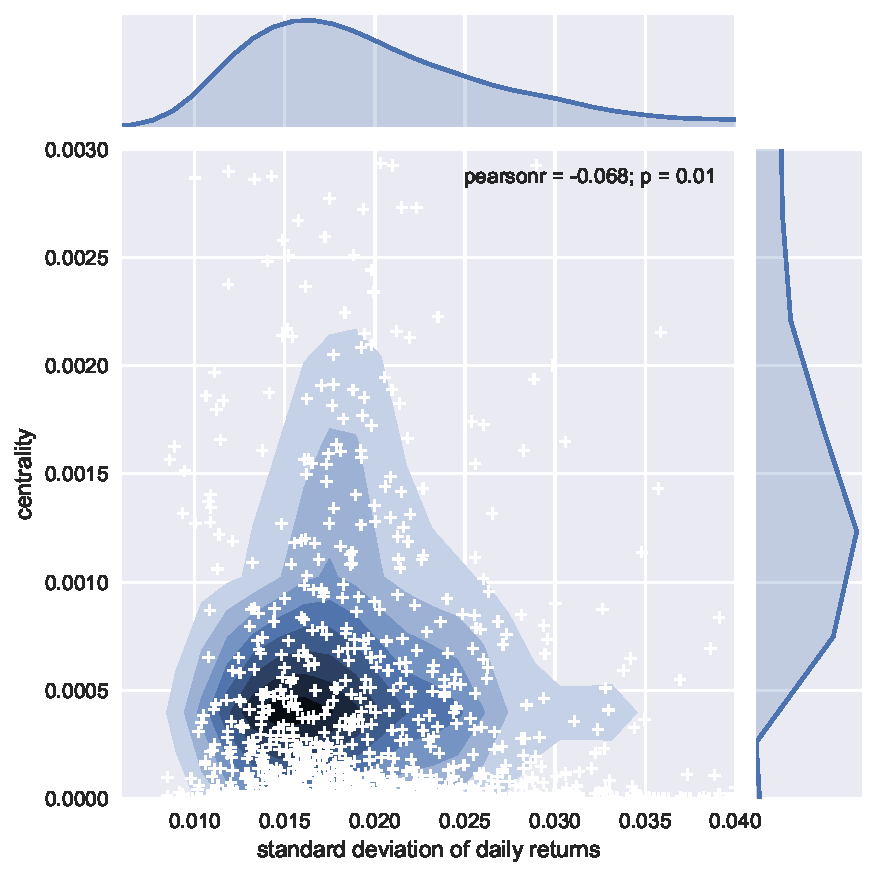
\includegraphics[width=10cm]{std_return_centrality} }
	
	\caption{Bivariate distribution}
	\label{fig:bivariate}
\end{figure}

% Assortativity with weight 0.12444731038165072



% Topological robustness
% Abnormal return regression with topological features as factors
\subsection{Analysis on the relationship between price return and clustering coefficient}


%\section{Community detection}
%\label{sec:community}
%命名各个community
\section{Stability of network}

%Industry


\chapter[Conclusions]{Conclusions and future work}
\label{cpt:conclude}
\section{Summary of results}
This thesis studied the directed complex networks of US stock market in 2016. The directions and weights of edges are determined by the economical transaction relations and stock price correlation coefficients respectively. Overall, the characteristics of topology properties have not changed significantly from undirected weighted stock networks from other literatures which used correlation coefficients of stock prices as the weights of edges. However, from the new horizon, this paper is able to analyse on a higher dimensionality -- topological property research and community detection with methods for directed networks which utilised the feature of edge directions. The resulting features of power-law and small-world for directed stock complex networks show continuity with the results in undirected stock complex networks researches. The study on community detection suggests "livelihood" and "production" are the most dominant and influential sectors in the stock market and the "finance" sector has extremely strong internal connections. The partitioned communities are highly related with the economical activities among industries and indicate the potential cascading impact from a collapse of a specific firm or sector. The theoretical and practical contributions of aforementioned findings have been discussed.

% This thesis has found the directed stock network is consistent with the undirected-weighted networks about some important topological properties in previous studies, i.e, they are both small-world and scale-free. The study on community detection suggests "livelihood" and "production" are the most dominant and influential sectors in the stock market and the "finance" sector has extremely strong internal connections. This thesis also has found that there is significant negative relationship between standard deviation of stock price return and its corresponding betweenness centrality. 
% theoretical and practical

\section{Future work}
In terms of future work, stock complex networks during a longer range of years can be generated and compared in together, the periods correspond to bull, bear, and stable market can be recognised and analysed separately and accordingly. New methods for determining the directions of edges to generate directed complex networks are expected to be proposed.

\chapter{Making a bibliography}
\label{cha:bib}
Whenever you wish to refer to books or articles relevant to your report
you should use a citation such as \cite{lamport}. You can also force
entries to appear in the bibliography without  a citation appearing in
the document, by using \verb=\nocite=.  

%% This nocite produces 2 entries in the bibliography
\nocite{boyle,rd-only} 

Each document cited must have an entry in a \textsf{.bib} file. For this
document we have only one, called \textsf{refs.bib}. These files are
listed in the \verb=\bibliography= command at the end of
\textsf{report.tex}. Note that the \textsf{.bib} files can (and often
do) contain many more entries than are actually cited in a partcular
document; the only ones that appear in the bibliography are those that
have been referenced using \verb=\cite= or \verb=\nocite=.

In order to generate the appropriate reference entries, you will need
to run \texttt{bibtex} after \texttt{latex} has been run, using the
command \texttt{bibtex report}. This will generate a file
\textsf{report.bbl}, which contains the bibliography entries. Once
that file is there, you do not need to run \texttt{bibtex} again
unless you add new citations, but you will probably have to run
\texttt{latex} twice after running \texttt{bibtex} the first time.

The \TeX{} FAQ (\cite{url-cite}) gives tips on how to cite URLs.

The file \textsf{refs.bib} provides an example of what can be done
with Bib\TeX. You can find much more information in any book on
\LaTeX, for example \cite{huang2009network,PhysRevLett.100.118703,CHOPRA2015865,CHEN2015224}

% Local Variables: 
% mode: latex
% TeX-master: "report"
% End: 


  \bibliography{refs}    % this causes the references to be listed

\bibliographystyle{alpha}
%% the bibliography style determines the format  in which both citations and references are printed,
%% other possible values are plain and abbrv
%%
%% If you want more control of the format of your citations you might want to take a look at
%% natbib.sty, which should be part of any standard LaTeX installation
%%
%% University regulations simply require that your citation style be consistent, so see what style
%% your supervisor recommends.

% Appendices start here

\appendix
\chapter{Example of operation}

An appendix is just like any other chapter, except that it comes after
the appendix command in the master file.

One use of an appendix is to include an example of input to the system
and the corresponding output.

One way to do this is to include, unformatted, an existing input file. 
You can do this using \verb=\verbatiminput=. In this appendix we
include a copy of the C file \textsf{hello.c} and its output file
\textsf{hello.out}. If you use this facility you should make sure that
the file which you input does not contain \texttt{TAB} characters,
since \LaTeX\ treats each \texttt{TAB} as a single space; you can use
the Unix command \texttt{expand} (see manual page) to expand tabs into
the appropriate number of spaces. 

\section{Example input and output}
\label{sec:inp-eg}
\subsection{Input}
\label{sec:input}
(Actually, this isn't input, it's the source code, but it will do as
an example)

\verbatiminput{hello.c}

\subsection{Output}
\label{sec:output}

\verbatiminput{hello.out}
\subsection{Another way to include code}
You can also use the capabilities of the \texttt{listings} package to
include sections of code, it does some keyword highlighting.

\lstinputlisting[language=C]{hello.c}

% Local Variables: 
% mode: latex
% TeX-master: "report"
% End: 


\end{document}
